% *****************************************************************************
%
%        FASThesis Manual
%        (FASThesis Class File Documentation)
%
%        Faculty of Applied Sciences
%        University of West Bohemia
%
%        Manual & Explanatory Document
%        Copyright (c) 2022-2024 Kamil Ekštein, Dept. of Computer Science
%        and Engineering, Faculty of Applied Sciences, UWB
%
%        Version:  0.96
%		 Encoding: UTF-8
%		 TeXer:    pdflatex
%
%        Last modification on 11-Apr-2024 by KE
%
% *****************************************************************************

% _____________________________________________________________________________
%
%
%	     DOCUMENT HEADER
%
% _____________________________________________________________________________
%
\documentclass[czech, ma, kiv, he, iso690alph, pdf, viewonly]{fasthesis}
\title{Generování jednotkových testů s využitím LLM}
\author{Milan}{Horínek}{Bc.}{}
\supervisor{Ing. Richard Lipka, Ph.D.}
\stagworkid{12345}% <== the unique identifier of the work in the STAG information system
\assignment{zadani.pdf}
\signdate{14}{05}{2024}{Plzeň}% <== the longest local name in the Czech Rep.

\usepackage[acronym]{glossaries}
\usepackage{pdflscape}
\usepackage{multirow}
\usepackage{float}
\usepackage{tikz}

\lstset{style=FASThesisLstStyle, numberblanklines=false, tabsize=5, keywordstyle=\color{red}}
\usetikzlibrary{shapes.geometric, arrows}

\tikzstyle{startstop} = [rectangle, rounded corners, minimum width=3cm, minimum height=1cm, text centered, draw=black, fill=red!30]
\tikzstyle{io} = [trapezium, trapezium left angle=70, trapezium right angle=110, minimum width=3cm, minimum height=1cm, text centered, draw=black, fill=blue!30]
\tikzstyle{process} = [rectangle, minimum width=3cm, minimum height=1cm, text centered, draw=black, fill=orange!30]
\tikzstyle{decision} = [diamond, minimum width=3cm, minimum height=1cm, text centered, draw=black, fill=green!30]
\tikzstyle{arrow} = [thick,->,>=stealth]

% Slovník
\makeglossaries
\newacronym{put}{PUT}{Parameterized Unit Test}
\newacronym{gui}{GUI}{Graphical User Interface}
\newacronym{gguf}{GGUF}{GPT-Generated Unified Format}
\newacronym{ggml}{GGML}{GPT-Generated Model Language}
\newacronym{ml}{ML}{Machine Learning - strojové učení}
\newacronym{vcs}{VCS}{Version Control System}
\newacronym{rnn}{RNN}{Recurrent Neural Network - Rekurenční neuronová síť}
\newacronym{cnn}{CNN}{Convolutional Neural Network - Konvoluční neuronová síť}
\newacronym{tdd}{TDD}{Test Driven Development - Vývoj řízený testy}

\newglossaryentry{llm}{
  name={LLM},
  description={Velký jazykový model (LLM - large language model) je typ modelu strojového učení, který je navržen tak, aby rozuměl a generoval text v přirozeném jazyce. Tyto modely jsou trénovány na obrovských datasetech a jsou schopny provádět různé úkoly, jako je textová klasifikace, generování textu, strojový překlad a další}
}

\newglossaryentry{testsmells}{
  name={testové pachy},
  description={Unit Test Smells jsou špatné návyky nebo postupy, které se mohou objevit při psaní jednotkových testů. Tyto "smelly" často vedou k neefektivním nebo nespolehlivým testům a mohou ztížit údržbu testovacího kódu. Příklady zahrnují Duplicated Asserts, Empty Tests a General Fixture},
}

\newglossaryentry{kontrakt}{
  name={kontrakt},
  plural={kontrakty},
  description={V kontextu jednotkových testů odkazuje na formálně definované podmínky nebo pravidla, které musí být dodrženy během vykonávání kódu. Kontrakty mohou specifikovat, co funkce očekává od svých vstupů a jaké výstupy nebo stavy by měla produkce kódu způsobit. Použití kontraktů pomáhá zajistit, že kód se chová podle očekávání a usnadňuje identifikaci chyb, když tyto podmínky nejsou splněny}
}

\newglossaryentry{filtr}{
  name={filtr},
  plural={filtry},
  description={Ve vývoji softwaru a testování se odkazuje na mechanismy nebo kritéria používaná k selektivnímu výběru testovacích vstupů nebo k rozhodování, které výstupy testů jsou relevantní pro další analýzu. Filtry mohou být použity k odstranění redundantních, nelegálních nebo jinak nežádoucích vstupů z procesu generování testů, což zvyšuje efektivitu testování tím, že se zaměřuje pouze na vstupy, které mohou odhalit chyby nebo porušení kontraktů}
}

\newglossaryentry{temperature}{
    name={teplota},
    plural={teploty},
    description={V terminologii strojového učení se jedná o hyperparametr, který ovládá reativitu a náhodnost vstupu modelu. Vyšší teplota vede k méně předvídatelným a kreativnějším výsledkům, kdežto nižší teplota produkuje více konzervativnější výstup.}
}

\newglossaryentry{context}{
    name={kontext},
    description={Rozsah textu nebo dat, který může model zpracovat při generování odpovědí. Funguje jako krátkodobá paměť modelu a určuje, kolik informací může model vzít v úvahu při tvorbě odpovědí.}
}

\newglossaryentry{token}{
    name={token},
    plural={tokeny},
    description={V NLP oblasti se jedná o rozdělení sekvence textu na menší části (například slova, části slov, atd.).}
}

\newglossaryentry{lsp}{
    name={LSP},
    description={Language Server Protocol. Protokol pro jazykový server používaný pro validaci syntaxe, sémantiky nebo formátování zdrojového kódu. Často se pod tímto označením myslí i samotný jazykový sever, který se o tuto analýzu stará.}
}

\newglossaryentry{servlet}{
    name={servlet},
    description={Serverový programový modul napsaný v programovacím jazyce Java, který zpracovává požadavky klientů a implementuje rozhraní Servlet. Přestože servlety mohou reagovat na jakýkoli typ požadavku, nejčastěji se používají k rozšíření aplikací hostovaných webovými servery.}
}

\newglossaryentry{benchmark}{
    name={benchmark},
    description={Standardizovaný test nebo pokus určení k meření a srovnání výkonu sytémů, komponent či aplikací.}
}

\newglossaryentry{mock}{
    name={maketa},
    description={V kontextu testování jde o simulované objekty, které imituje chování reálných komponent v rámci systému a slouží k izolaci testované jednotky od jejích závislostí.}
}


\addbibresource{dp.bib}% <== the file with the bibliographical database to be used throughout the text
% _____________________________________________________________________________
%
%
%	     DOCUMENT FRONTMATTER TEXTS
%
% _____________________________________________________________________________
%
\abstract{TBD}
% *** English abstract ***
{TBD}
\keywords{LLM, testing, unit, Robot Framework}
% _____________________________________________________________________________
%
%        ACKNOWLEDGEMENT
% _____________________________________________________________________________
%
\acknowledgement{TBD}

% Gloss
\auxfrontmattercontent{
    \printglossary[type=\acronymtype,title=Zkratky]
    \printglossary[title=Slovník pojmů]
}
% _____________________________________________________________________________
%
%
%	     DOCUMENT TEXT BEGINNING
%
% ____________________________________________________________________________
%
\begin{document}
\frontpages[tm] % or notm if the `trademark' declaration is not needed
\tableofcontents
% 
% -x---- ADDITIONAL COLOUR DEFINITIONS ----------------------------------------
%
\makeatletter%
\ifx\FASThesis@style\c@fullcolor%
	\definecolor{fascolor}{cmyk}{0.06, 0.27, 1.0, 0.12}%
	\definecolor{fascolordk}{cmyk}{0.05, 0.28, 1.0, 0.24}%
\else%
	\definecolor{fascolor}{cmyk}{0, 0, 0, 0.6}%
	\definecolor{fascolordk}{cmyk}{0, 0, 0, 0.75}%
\fi%
\makeatother%
\lstdefinestyle{plainsrc}{
	backgroundcolor=\color{fascolor!10},
	basicstyle=\ttfamily\footnotesize,
	numberstyle=\tiny\color{fascolordk},
	numbers=left,
	numbersep=5pt,
	keepspaces=true,
	tabsize=2,
	extendedchars=true,
	literate={á}{{\'a}}1 {č}{{\v{c}}}1 {ď}{{\v{d}}}1 {é}{{\'e}}1 {ě}{{\v{e}}}1 {è}{{\`{e}}}1 {í}{{\'{\i}}}1 {ľ}{{\v{l}}}1 {ň}{{\v{n}}}1 {ó}{{\'o}}1 {ŕ}{{\'r}}1 {ř}{{\v{r}}}1 {š}{{\v{s}}}1 {ť}{{\v{t}}}1 {ú}{{\'u}}1 {ů}{{\r{u}}}1 {ý}{{\'y}}1 {ž}{{\v{z}}}1
	{Á}{{\'A}}1 {Č}{{\v{C}}}1 {Ď}{{\v{D}}}1 {É}{{\'E}}1 {Ě}{{\v{E}}}1 {È}{{\`{E}}}1 {Í}{{\'I}}1 {Ľ}{{\v{L}}}1 {Ň}{{\v{N}}}1 {Ó}{{\'O}}1 {Ŕ}{{\'R}}1 {Ř}{{\v{R}}}1 {Š}{{\v{S}}}1 {Ť}{{\v{T}}}1 {Ú}{{\'U}}1 {Ů}{{\r{U}}}1 {Ý}{{\'Y}}1 {Ž}{{\v{Z}}}1
}

\setlength{\parskip}{1em}
% -x---- END OF ADDITIONAL COLOUR DEFINITIONS ---------------------------------


\chapter{Úvod}
    TDB - Co jsou unit testy, LLM, a jejich předpoklady, GUI testování

    Něco na úvod
    
    \section{Testy}

    \section{Jazykové modely}

    \section{Motivace}

\chapter{Rešerše} \label{sec:research}

    \section{Provedená práce v problematice} \label{sec:previouswork}
        \subsection{Předchozí automatizovaná řešení}
        Jazykové modely nebyli prvními pokusy o automatizované generování jednotkových testů. V sučasnosti existuje spousta metod, které se neustále rozvíjejí a nové vznikají. Mezi ně patří příklady jako \textit{fuzzing, generování náhodných testů řízených zpětnou vazbou, dynamické symbolické vykonání, vyhledávvací a evoluční techniky, parametrické testování}. Zároveň také již na počátku století byly pokusy o vytvoření vlastní neuronové sítě sloužící právě čistě k úkolu testování softwaru (například článek "Using a neural network in the software testing process"). \cite{Vanmali2002UsingAN} V této sekci je ukázka několika z nich. 

        \subsubsection{Programatická řešení}
        Jedna z používaných programatických automatizovaných metod pro tvrobu jednotkových testů je tzv. \textit{fuzzing}. V rámci těchto testů musí uživatel stále definovat jeho kódovou strukturu, resp. akce, které test bude provádět a jaký výstup očekávat. Automaticky generovaný je pouze vstup tohoto testu. Výhodou zde tedy je, že uživatel nemusí vytvářet maketu vstupních dat testu, která se zde vytvoří automatizovaně. Zůstává zde však problematika, že pro uživatele není kód \emph{black-box}, ale celou jeho strukturu včetně požadovaného výstupu musí sám definovat. \cite{fuzzing}

        Pouze vstupy dokáže také generovat metoda \textit{symbolického vykonání}, která postupně analyzuje chování větvení programu. Začíná bez předchozích znalostí a používá řešitel omezení (anglicky označovaný jako \textit{constraint solver}) k nalezení vstupů, které prozkoumají nové vykonávací cesty (anglicky \textit{execution path}) v rámci řízení toku programu. Jakmile jsou testy spuštěny s těmito vstupy, nástroj sleduje cestu, kterou se program ubírá, a aktualizuje svou znalostní bázi \((q)\) s novými podmínkami cesty \((p)\). Tento iterativní proces se opakuje a nadále zpřesňuje sadu známých chování a snaží se maximalizovat pokrytí kódu. \textit{Známé chování} lze definovat jako sadu identifikovaných vykonávacích cest programu, včetně podmínek a stavů, které byly analyzovány a uloženy do znalostní báze nástroje \((q)\). Umožňuje efektivně generovat nové testovací vstupy a předvídat chování programu na základě již známých dat. Nástroje běžně zvládají různé datové typy a respektují pravidla viditelnosti objektů. Snaží se také používat mock objekty a parametrizované makety k simulaci různých chování vstupů, čímž zlepšuje proces generování testů, aby odhalila potenciální chyby a zajistila komplexní pokrytí kódu testy. \cite{parizek_symbolic_execution} Tato metoda je implementována například v nástroji IntelliTest v rámci IDE \textit{Visual Studio}. Je používáná v kombinaci s \emph{parametrickými testy}, také označovanými jako \acrshort{put}. Na rozdíl od tradičních jednotkových testů, které jsou typicky uzavřené a nezměnitelné metody, parametrické testy mohou přijímat libovolné množství parametrů a adaptují se tak testovacím scénářům. Software pro jejich vytváření se pak snaží automaticky generovat (minimální) sadu vstupů, které plně pokryjí kód dosažitelný z testu. Nástroje jako např. \textit{IntelliTest} automaticky generují vstupy pro \acrshort{put}, které pokrývají mnoho vykonávacích cest testovaného kódu. Každý vstup, který pokrývá jinou cestu, je "serializován" jako jednotkový test. Parametrické testy mohou být také generické metody (funkce schopná pracovat s různými druhy datových typů bez nutnosti psát pro každý typ specifický kód zvlášť), v tom případě musí uživatel specifikovat typy použité k instanci metody. Testy také mohou obsahovat atributy pro \emph{očekávané} (např. dělení nulou) a případně \emph{neočekávané} vyjímky (např. předání reference na nulový objekt). Neočekávané vyjímky vedou k selhání testu. \acrshort{put} tedy do velké míry redukují potřebu uživatelského vstupu pro tvorbu jednotkových testů. \cite{IntelliTestInputGeneration2023} \cite{microsoft2023testgen}

        Pokud zvolíme symbolické řešení vstupu (některé vstupní argumenty testovaného programu nebudou reprezentovány konktrétními hodnotami, ale zastoupené symbolickými proměnnými) společně s determinovanými vstupy (využity konkrétní hodnoty) a vykonávací cestou, vzniká tak hybridní řešení zvané jako \emph{konkolické testovaní} nebo \emph{dynamické symbolické vykonání}. Tento druh testů dokáží tvořit nástroje jako \textit{SAGE, KLEE} nebo \textit{S2E}. Problémem tohoto přístupu však je, když program vykazuje \emph{nedeterministické} chování, kdy tyto metody nebudou schopny určit správnou cestu a zároveň tak ani zaručit dobré pokrytí kódu/větví. Nedeterministické chování není tolik obvyklé a objevuje se zejména v případě \textit{paralelizmu}, \textit{externího přerušení} či u algortimů postavených na \textit{pseudonáhodě}. \cite{ncatlab_nondeterministic_computation} Tento problém není speficický pouze pro tento typ automatizovaného testování, ale i pro předchozí varianty. Zatímco \emph{symbolická} část vykonání objeví veškeré možné cesty, \emph{konkrétní} vykonání poté určí sled jednotlivých událostí při spuštění, aby nedocházelo k redundantnímu testování. \cite{aldrich2019concolic} Dalším problémem této metody také může být výběr stavových proměnných. Problémem je zejména jejich rozsah. Například více stavových proměnných s malým celočísleným rozsahem povede pouze k omezenému množství cest, kdežto pouze jednotky takových proměnných o celém rozsahu typu \verb|double| může vést k daleko vyššímu počtu cest, což také zvýší výpočetní náročnost těchto metod a tedy se i snižuje pravděpodobnost úspěšného nenalezení praktického řešení (v případě, že takové řešení vůbec existuje nebo je to účelem vyhledávání). \cite{concolic_chalenges_2019} \cite{engler2006exe} \cite{sen2005cute} \cite{zhou2006safedrive}

        Další metodou je \textit{náhodné generování testů řízené zpětnou vazbou}, která je vylepšením pro generování náhodných testů tím, že zahrnuje zpětnou vazbu získanou z provádění testovacích vstupů v průběhu jejich vytváření. Tato technika postupně buduje vstupy tím, že náhodně vybírá metodu volání (jedná se o dostupnou funkci nebo metodu v rámci programu) a hledá hodnoty argumentů, které náhodně generuje nebo upravuje vstupy vytvořenými v předchozích iteracích tohoto procesu. Jakmile dojde k sestavení vstupu, je provedeno jeho vykonání a výsledek ověřen proti sadě \gls{kontrakt}ů a \glspl{filtr}ů. Výsledek vykonání jeho srovnáním s očekávanými výstupy, definovanými v kontraktu, a filtry určuje, zda je vstup redundantní (definován tak filtry), proti pravidlům (jak filtrů tak kontraktů), porušující \gls{kontrakt} (např. nedefinované výstupy) nebo užitečný pro generování dalších vstupů (splňuje konktrakt a prochází filtry). Technika vytváří sadu testů, které se skládají z jednotkových testů pro testované třídy. Úspěšné testy mohou být použity k zajištění faktu, že \glspl{kontrakt} kódu jsou zachovány napříč změnami programu; selhávající testy (porušující jeden nebo více kontraktů) ukazují na potenciální chyby, které by měly být opraveny. Tato metoda dokáže vytvořit nejen vstup pro test, ale i tělo (kód) testu. Ovšem pro uživatele je stále vhodné znát strukturu kódu. \cite{FeedbackDirectedRT}

        Z programatických metod se zdají být nejpokročilejší \emph{evoluční algoritmy} pro generování sad jednotkových testů, využívající přístup založený na vhodnosti, aby vyvíjely testovací případy, které mají za cíl maximalizovat pokrytí kódu a detekci chyb. Tyto algoritmy mohou autonomně generovat testovací vstupy, které jsou navrženy tak, aby prozkoumávaly různé vykonávací cesty v aplikaci. Uživatelé mohou interagovat s vygenerovanými testy jakožto s \textit{black-boxem}. Testy se zaměřují na vstupy a výstupy, aniž by potřebovali rozumět vnitřní logice testovaného systému. Tento aspekt evolučního testování je zvláště výhodný při práci se složitými systémy nebo když zdrojový kód není snadno dostupný. Proces iterativně upravuje testovací případy na základě pozorovaných chování, upravuje vstupy pro efektivnější prozkoumání systému a identifikaci potenciálních defektů. Tato metoda podporuje vysokou úroveň automatizace při generování testů, snižuje potřebu manuálního vstupu a umožňuje komplexní pokrytí testů s menším úsilím. \cite{CAMPOS2018207} \cite{abs-2111-05003}

        \subsubsection{Neuronové sítě}
        Ke generování jednotkových testů lze využít i vlastní neuronové sítě. Takové se pokoušeli vytvářet například v práci "Unit test generation using machine learning"\cite{Saes2018UnitTestGeneration}, kde byly testovány primárně RNN a experimentálně CNN sítě (ty však měli problém s větším množstvím tokenů). Modely byli testovány na jazyce Java. Metoda přistupovala k programům jakožto white box, tedy měli k dispozici celý zdrojový kód včetně zkompilovaného bytecodu. Při nejlepší konfiguraci dosáhl výsledek modelu \(70.5\%\) parsovatelného kódu (tedy takového bez chyb) natrénovaný z bezmála 10000 příkladů \textit{zdrojový kód - test}. Výsledek práce je však stále jakýsi "proof of concept", protože zatímco vygenerují částečně použitelný výsledek, je vždy nutný zásah experta, aby mohlo dojít k vytvoření celého testovacího souboru. Takovéto sítě se však mohou silně hodit jako výpomoc programátorovi při psaní testů.

        \subsubsection{Nevýhody současných metod}
        Současné metody generování jednotkových testů, jako je \textit{fuzzing} a \textit{symbolické vykonání}, často vyžadují podrobnou znalost struktury kódu a očekávaných výstupů, což omezuje jejich efektivitu a zvyšuje složitost tvorby testů. Jen některé z těchto metod jsou schopné vygenerovat testy pouze na bázi specifikace (z black box pohledu) bez vnitřní znaloasti kódu. Většina z klasických metod je zároveň schopna generovat pouze vstupy jednotkových testů, ale už ne samotné tělo (kód) testu nebo očekávané výstupy, a tedy pouze složí jako jakási konstra pro programátora, který musí test doimplementovat.

        Velké jazykové modely (\gls{llm}) mohou být atraktivní alternativou, protože pomocí nich lze potenciálně automatizovat generování jak vstupů pro testy, tak přidruženého testovacího kódu, čímž se snižuje potřeba hlubokého porozumění struktuře kódu. S takovým nástrojem není potřeba programátora, ale může s ním pracovat i méně zkušený uživatel (např. \textit{tester}). Dále je zde možnost otestovat kód za pomocí slovní specifikace pro funkci nebo vlastnosti. Takové specifikace se používají napřílad v \textit{aero-space} nebo \textit{automotive} sektoru. \GLS{llm} také mohou objevit všechny možné stavy, které mohou u vstupu nebo výstupu nastat a pokusit se pro ně navrhnout test.

    \subsection{Vydané publikace}
    Jeden z poměrně nedávno vydaných článků (září 2023) nazvaný "An Empirical Evaluation of Using Large Language Models for Automated Unit Test Generation" \cite{schafer2023empirical} se zabývá využitím velkých jazykových modelů (\gls{llm}) pro automatizované generování jednotkových testů v jazyce JavaScript. Implementovali nástroj s názvem \textbf{TESTPILOT}, který využívá \gls{llm} \textit{gpt3.5-turbo}, \textit{code-cushman-002} od společnosti OpenAI a  také model StarCoder, který vznikl jako komunitní projekt \cite{StarCoder2023}. Vstupní sada pro \gls{llm} obsahovala signatury funkcí, komentáře k dokumentaci a příklady použití. Nástroj byl vyhodnocen na 25 balíčcích npm obsahujících celkem 1684 funkcí API. Vygenerované testy dosáhly pomocí gpt3.5-turbo mediánu pokrytí příkazů 70,2\% a pokrytí větví 52,8\%, čímž překonaly nejmodernější techniku generování testů v jazyce JavaScript zaměřenou na zpětnou vazbu, Nessie.

    Zmíněný model \emph{StarCoder} byl představen v článku "StarCoder: may the source be with you!" \cite{StarCoder2023} z května 2023. Vytvořeny byly konkrétně 2 verze, \textit{StarCoder} a \textit{StarCoderBase}, s 15,5 miliardami parametrů a délkou kontextu 8K. Tyto modely jsou natrénovány na datové sadě nazvané \textit{The Stack}, která obsahuje 1 bilion tokenů z permisivně licencovaných repozitářů GitHub. \textit{StarCoderBase} je vícejazyčný model, který překonává ostatní modely open-source \gls{llm} modely, zatímco \textit{StarCoder} je vyladěná verze speciálně pro Python, která se vyrovná nebo překoná stávající modely zaměřené čistě na Python. Článek poskytuje komplexní hodnocení, které ukazuje, že tyto modely jsou vysoce efektivní v různých úlohách souvisejících s kódem.

    Článek "Exploring the Effectiveness of Large Language Models in Generating Unit Tests" \cite{siddiq2023exploring} z dubna 2023 hodnotí výkonnost tří \gls{llm} - \textit{Codex}, \textit{CodeGen} a \textit{GPT-3.5} - při generování jednotkových testů pro třídy jazyka Java. Studie používá jako vstupní sady dva benchmarky, \href{https://paperswithcode.com/dataset/humaneval-x}{HumanEval} a \href{https://paperswithcode.com/dataset/evosuite-sf110-benchmark}{Evosuite SF110}. Klíčová zjištění ukazují, že \textit{Codex} dosáhl více než 80\% pokrytí v datové sadě \textit{HumanEval}, ale žádný z modelů nedosáhl více než 2\% pokrytí v benchmarku \textit{SF110}. Kromě toho se ve vygenerovaných testech často objevovaly tzv. \gls{testsmells}, jako jsou \textit{duplicitní tvrzení} a \textit{prázdné testy} \cite{testsmells}.

    \subsubsection{Srovnání výsledků}
    Výsledky diskutovaných studií v předchozím bodě jsme srovnali v tabulce \ref{tab:paper_comp}. V rámci první práce dosahuje nejlepších výsledků model \textit{gpt-3.5-turbo}, který dosáhl 70\% pokrytí kódu testy a 48\% úspěšnosti testů. U druhé studie má tento model na testovací sadě \textit{HumanEval} velice podobný výsledek, ovšem model \textit{Codex} dosáhl lepších výsledků. Může však také jít o rozdíl způsobený programovacím jazykem. Zatímco v práci \cite{schafer2023empirical} se využívá jako benchmark sada balíčků jazyka \textit{JavaScript}, který kvůli absenci explicitního typování, může být obtížnější pro strojové testování oproti jazyku Java, který je využit ve zbylých 2 pracích. \cite{jutai} také využívá Javu a s modelem \textit{gpt-3.5-turbo} dosahuje podobného pokrytí kódu a úspěšnosti jako \textit{Codex} v práci \cite{siddiq2023exploring}.


    \subsection{Modely} \label{sec:research_models}
    % TODO Tady asi nějaká předmluva k těm modelům a co za modely se vlastně používá 
    Na \GLS{llm} modelech nás konkrétně zajímá schopnost pozorumět progamovacím jazykům a ty poté také generovat na výstupu. Důležité pro nás také je, zda daný model je proprietární či otevřený a pod jakou licencí, tedy zda by byl vhodný pro naši práci. V případě analýzy zdrojového kódu může být také klíčovou vlastností délka kontextu daného modelu. Tyto vlastnosti jsou také zaneseny do tabulky \ref{tab:code_models_comp}.

    \paragraph{StarCoder} Jedním z často používaných modelů v předchozích pracích je \textit{StarCoder} a \textit{StarCoderBase}, diskutovaný již v sekci \ref{sec:previouswork}. \textit{Base} verze je schopna generovat kód pro více jak 80 programovacích jazyků. Model je navržen pro širokou škálu aplikací obsahující \textit{generování}, \textit{modifikaci}, \textit{doplňování} a \textit{vysvětlování} kódu. Jeho distribuce je volná a licence \textbf{CodeML OpenRAIL-M 0.1} \cite{BigCode2023} umožňuje ho využívat pro množštví aplikací včetně komerčních nebo edukačních. Jeho uživatel však má povinnost uvádět, že výsledný kód byl vygenerován modelem. Licence má své restrikce z obavy tvůrců, protože by model mohl někoho při nepsrávném použití ohrozit. Tyto restrikce se aplikují na na všechny derivace projektů pod touto licencí. Zároveň není kompatibilní s Open-Source licencí právě kvůli těmto restrikcím.

    Model StarCoder se také dočkal novější verze \textit{StarCoder2}, který nepřímo navazuje na model \textit{StarCoderBase}. Je naučen na archivu GitHub repoziářů archivovaných v rámci organizace \textit{Software Heritage}, čítajících přes 600 programovacích jazyků a dalších pečlivě vybraných dat jako například \textit{pull requesty}. Mimo toho také trénovací data obsahují staženou dokumentaci k vybraným projektům. Model se vyjímá tím, že se snaží udržet malou velikost. Je nabízen ve verzích s \textit{3, 7} a \textit{15} miliardy parametrů, i přesto však dle jejich úvodní studie \cite{lozhkov2024starcoder} nabízí na sadě populárních programovacích jazyků shodné či lepší výsledky oproti modelu \textit{CodeLlama} s 34 miliardy parametrů. Výhodou tohoto modelu nepochybně je, že ho lze spustit na spoustě dnešních počítačů s plným offloaded na grafickou kartu.

    \paragraph{CodeLlama} Nedávno vydaným modelem je \textit{Code Llama} od společnosti Meta. Jedná se o evoluci jejich jazykového modelu \textit{Llama} specializovaný však čistě na úlohy kódování. Je postaven na platformě \textit{Llama 2} a existuje ve třech variantách: \textit{základní Code Llama}, \textit{Code Llama - Python} a \textit{Code Llama - Instruct}. Model podporuje více programovacích jazyků, včetně jazyků jako Python, C++, Java, PHP, Typescript, C# nebo Bash. Je určen pro úlohy, jako je generování kódu, doplňování kódu a ladění. Code Llama je zdarma pro výzkumné i komerční použití a je uvolněn pod licencí MIT. Uživatelé však musí dodržovat  zásady přijatelného použití, ve kterých je uvedeno, že model nelze použít k vytvoření služby, která by konkurovala vlastním službám společnosti Meta. 

    \paragraph{Copilot} Velmi populárním nástrojem pro generování kódu za pomocí \gls{llm} je \href{https://github.com/features/copilot}{GitHub Copilot}, který je postaven na modelu \textit{codex} od OpenAI. Původní model však byl přestal být zákazníkům nabízen a namísto něj OpenAI doporučuje ke generování kódu využívat chat verze modelů GPT-3.5 a GPT-4. Na architektuře GPT-4 je také postavený nástupce služby Copilot, \href{https://github.com/features/preview/copilot-x}{Copilot X}. Zmíněné modely chat GPT-3.5 a GPT-4 jsou primárně určeny pro generování textu formou chatu. Zvládají však zároveň i dobře generovat kód a jsou vhodné i úlohu generování jednotkových testů. Narozdíl od předchozích modelů však nejsou volně distribuovány a jsou poskytovány pouze jako služba společností OpenAI skrze API nebo je lze hostovat v rámci služby Azure společnosti Microsoft, která zajišťuje větší integritu dat. Jedná se tedy o uzavřený model a jeho uživatelé musí souhlasit s jeho podmínkami použití.

    %TODO Existují i další modely, co by bylo super přidat

        \newpage

        \begin{landscape}
            \centering
            \begin{table}[H]
                \begin{tabular}{|p{6cm}|c|c|c|c|}
                    \hline
                    \textbf{Práce} & \textbf{Model} & \textbf{Benchmark} & \textbf{Pokrytí testy} & \textbf{Úspěšnost} \\
                    \hline
                    \multirow{3}{6cm}{An Empirical Evaluation of Using Large Language Models for Automated Unit Test Generation} & \textit{gpt-3.5-turbo} & \multirow{3}{*}{Sada NPM balíčků} & 70.2\% & 48\% \\
                     & \textit{code-cushman-002} & & 68.2\% & 47.1\% \\
                     & \textit{StarCoder} & & 54\% & 31.5\% \\
                    \hline
                    \multirow{6}{6cm}{Exploring the Effectiveness of Large Language
Models in Generating Unit Tests} & \multirow{2}{*}{\textit{gpt-3.5-turbo}} & HumanEval & 69.1\% & 52.3\% \\
                     & & SF110 & 0.1\% & 6.9\% \\
                     & \multirow{2}{*}{\textit{CodeGen}} & HumanEval & 58.2\% & 23.9\% \\
                     & & SF110 & 0.5\% & 30.2\% \\
                     & \multirow{2}{*}{\textit{Codex (4k)}} & HumanEval & 87.7\% & 76.7\% \\
                     & & SF110 & 1.8\% & 41.1\% \\
                    \hline
                    Java Unit Testing with AI: An AI-Driven Prototype for Unit Test Generation & \textit{gpt-3.5-turbo} & JUTAI - Zero-shot, temperature: \(0\) & 84.7\% & 71\% \\
                    \hline
                \end{tabular}
                \centering
                \caption{Přehled a srovnání studií}
                \label{tab:paper_comp}
            \end{table}
            \begin{table}[H]
                \begin{tabular}{|c|c|c|c|c|c|}
                    \hline
                    \textbf{Model} & \textbf{Otevřenost} & \textbf{Licence} & \textbf{Počet parametrů} & \textbf{Počet programovacích jazyků} & \textbf{Datum vydání} \\
                    \hline
                    \textit{StarCoderBase} & Volně dostupný & CodeML OpenRAIL-M 0.1 & 15.5 miliardy & 80+ & 5/2023 \\
                    \hline
                    \textit{Code Llama} & Volně dostupný & Llama 2 Licence & 34 miliard & 8+ & 8/2023 \\
                    \hline
                    \textit{gpt-3.5-turbo} & Uzavřený & Proprietární & 175 miliard? & ? & 5/2023 \\
                    \hline
                    \textit{gpt-4} & Uzavřený & Proprietární & 1.76 bilionu & ? & 3/2023 \\
                    \hline
                \end{tabular}
                \centering
                \caption{Přehled a srovnání modelů generujících kód}
                \label{tab:code_models_comp}
            \end{table} 
        \end{landscape}
    
    \section{Testovací program} \label{sec:test_program}

    Pro účely této práce jsme se rozhodli vydat cestou \acrshort{gui} testů, konkrétně webových stránek / webové aplikace. Mezi požadavky na testovanou aplikaci a její výběr bylo mimo možnosti vytvořit pro ní automatiovanou sadu testů, také možnost zavedení (\emph{injekce}) chyb do aplikace, díky kterým bude možno ověřit nejen fakt, že vygenerované testy jsou schopné detekovat \textit{korektní} chování softwaru, ale také úspěšně detekovat \textit{chyby}. Volitelnou podmínkou také byla existence již existujících testů vytvořených lidským programátorem, se kterými by bylo možné strojově generované testy porovnat.
    
    Těmto požadavkům vyhovuje jeden z předešlých univerzitních projektů nazvaný \textbf{TbUIS} (\textit{Testbed University Information System}), na který vytvořili Matyáš a Šmaus pod vedením doc. Herouta. \cite{Matyas2018} \cite{Smaus2019} Aplikace představuje \textit{maketu} univerzitního informačního systému, avšak i tak implementuje většinu functionality, kterou bysme od podobného systému čekali a nabízí pohled jak ze strany \textit{studenta} tak ze strany \textit{vyučujícího} (viz obr. \ref{fig:tbuis}). Funkce tohoto systému vycházejí ze sady \textit{use casů}, které popisuje web \footnote{Aplikaci lze nalézt na adrese: \url{https://projects.kiv.zcu.cz/tbuis/web/}} aplikace. Výhodou tohoto systému primárně je, že nabízí nejen plně funkční a otestovanou variantu, ale také \(27\) dalších poruchových klonů, vždy porušující alespoň jeden \textit{use case} a s ním potenciálně spojený test.

    Projekt dále také obsahuje i sadu jak \textit{funkčních} testů primárně pro backend vytvořených Poubovou tak také \textit{akceptačních} testů držejících se pevně specifikací, vytvořených Vaisem. \cite{Poubova2019} \cite{Vais2020} Tyto testy využívají nejen pevné znalosti jednotlivých uživatelských scénářů, ale také jsou parametrizovány pomocí všech dostupných dat k aplikaci (\textit{např. uživatelská jména, předměty, zkoušky, atd.}) k vyhodnocení chování softwaru v co nejvíce případech. Právě \textit{akceptační} testy využívají námi zvolený \textbf{RobotFramework} pro testování a tedy vytvořené scénáře bude možné do určité míry přirovnat a případně zhodnotit jejich kvalitu. 

    \begin{figure}
        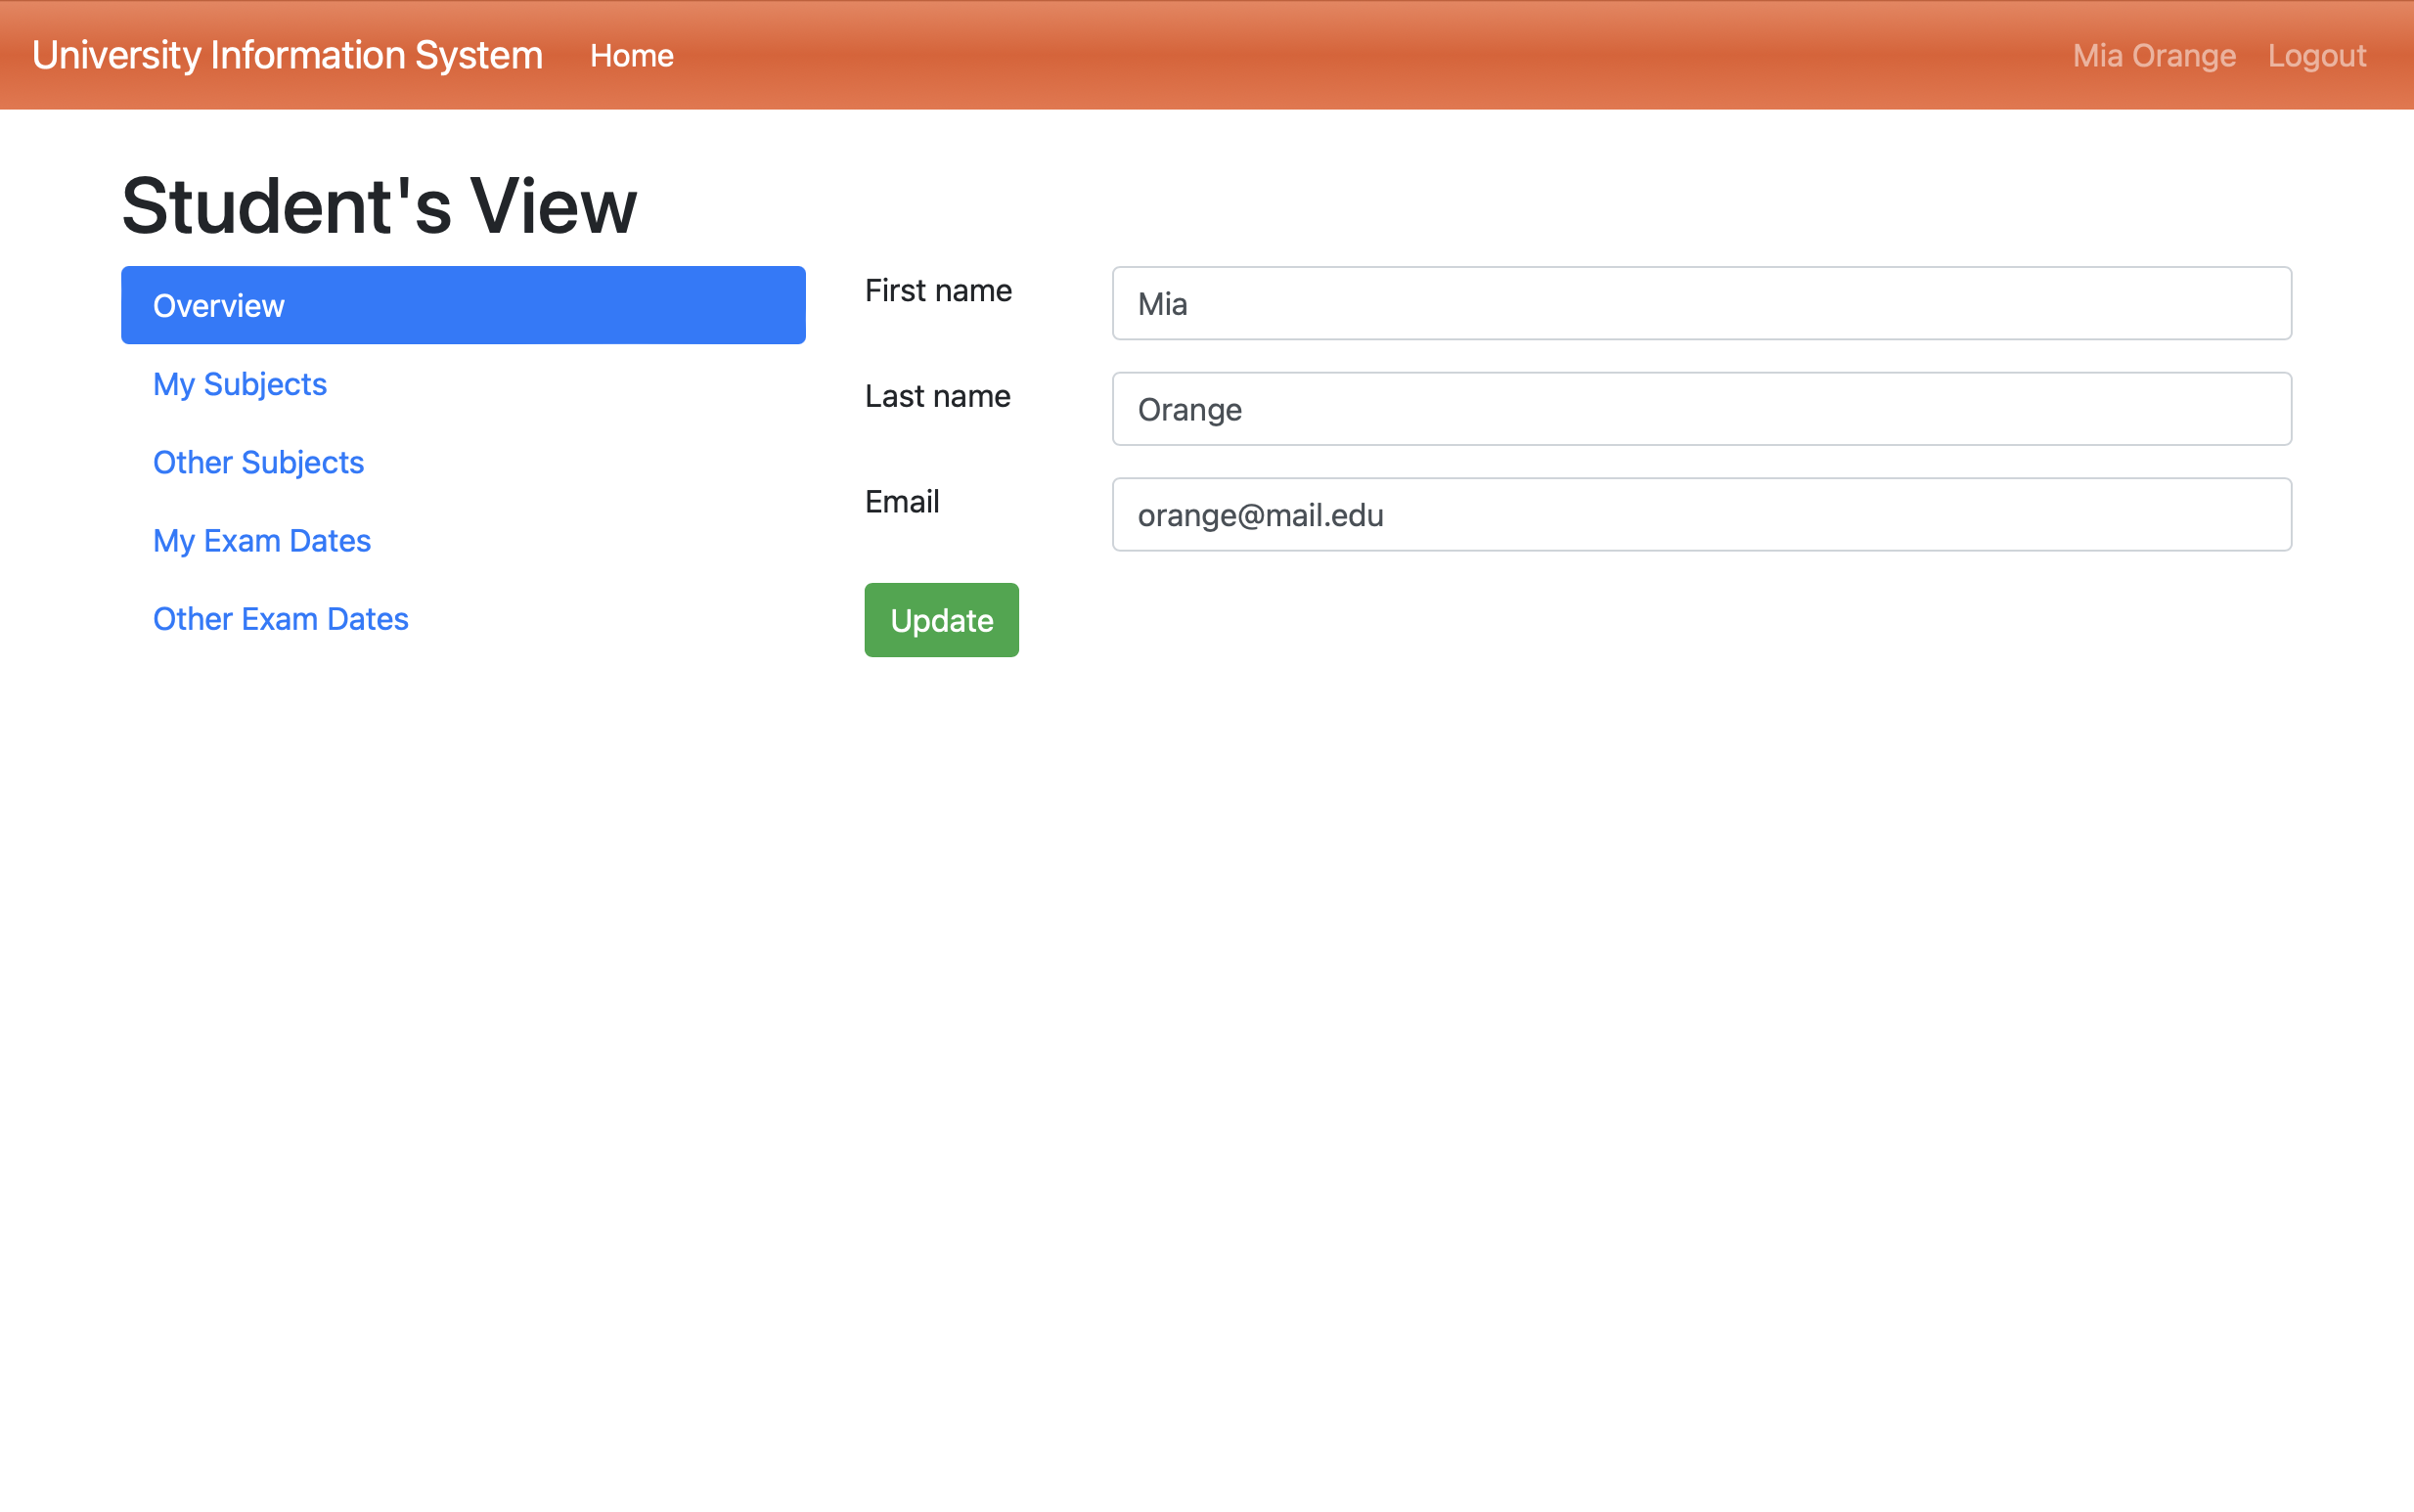
\includegraphics[width=0.8\textwidth]{pic/tbuis.png}
        \centering
        \caption{Prostředí systému TbUIS z pohledu studenta.}
        \label{fig:tbuis}
    \end{figure}

\chapter{Návrh}

        \section{Co a jak testujeme}

        \section{Navrhované řešení}


\chapter{Generování testů} \label{sec:test_generation}

    \section{Prerekvizity pro generování spuštění testů}
    %TODO Dopsat
    %TODO Je toto vhodné místo pro prerekvizity i když nesouvisí čistě jen s generováním testů?

    \section{Výběr scénářů} \label{sec:scenarios}

    Pro vygenerování testů za pomocí LLM bylo nejdříve nutné vybrat ze sady \textit{use caseů}\footnote{Seznam dostupný na adrese: \url{https://projects.kiv.zcu.cz/tbuis/web/page/uis#use-cases}} scénáře vhodné pro demonstraci nejen správné funkčnosti, ale také s možností ověření nesprávného chování na poruchových klonech (diskutováno v sekci \ref{sec:test_program}). Požadavek tedy byl, aby většina z vybraných scénářů vycházející z \textit{use casu} měl alespoň jeden poruchový klon, případně více. Vybráno bylo \(10\) scénářů, testovaných celkově na \(14\) variantách programu. Seznam vytvořených specifikací pro automatické generování testů se nachází v tabulkách \ref{tab:specs_1} a \ref{tab:specs_2}. Scénáře budou dále také referovány jako \textit{specifikace}. Každá specifikace má \textit{číslo}, které odpovídá číslu \textit{use casu}, ze kterého vychází (např. specifikace \(04\) vychází z use casu \textit{UC.04}). Zde je nutné poznamenat, že ne všechny specifikace vychází pevně z jejich use casů, ale byli upravené tak, aby šli provést v jednom chodu bez nutných závislostí (\textit{jako například namísto podmínky přihlášeného uživatele se uživatel vždy musí na začátku či během testu přihlásit do systému}). Popis specifikací v tabulce je pouze orientační a pro bližší upřesnění jednotlivých kroků, které se mají provést referujte web projektu. V tomto seznamu se také u každé specifikace nachází výčet klonů, na kterých lze očekávat poruchu. Celkový seznam klonů, a kterých se budou všechny vytvořené testy spouštět lze nalézt v tabulce \ref{tab:clones}. Podobně jako v případě specifikací, čísla klonů odpovídají číslům, jak jsou uvedena na oficiálním webu\footnote{Seznam poruchových klonů společně s možností stažení: \url{https://projects.kiv.zcu.cz/tbuis/web/page/download}} projektu společně s vysvětlením jednolivých chyb varianty. Pro přehlednost jsme bezchybnou variantu označili číslem \(00\).

    \begin{table}
        \begin{tabular}{|c|p{7cm}|c|}
            \hline
            \textbf{Specifikace} & \textbf{Popis} & \textbf{Porucha na klonech} \\
            \hline
            \(1\) & \textit{Přihlášení do aplikace} \newline Student i učitel se přihlásí do aplikace přihlašovacími údaji, dostupnými v databázi systému. Dále se zkontroluje, zda systém pro účet s neexistujícím uživatelským jménem nebo neplatným heslem vypíše chybovou hlášku. &  \(02\) \\
            \hline
            \(4\) & \textit{Odepsání předmětu} \newline Student se přihlásí, odepíše předmět v patřičné sekci systému. Předmět by následně měl zmizet v ostatních sekcích a to jak v pohledu studenta tak učitele. & \(04, 19, 25, 26, 28\) \\
            \hline
            \(6\) & \textit{Zapsání předmětu} \newline Student se přihlásí, zapíše předmět v patřičné sekci, který se následně zobarazí i v ostatních částech systému. Z učitelského pohledu by se student měl zobrazit na seznamu studentů daného předmětu. & \(25, 26, 28\) \\
            \hline
            \(8\) & \textit{Registrace na zkoušku} \newline Student se přihlásí do systémů a zapíše se na jeden z možných zkouškových termínů. Tento termín by se měl přesunout mezi již zapsané termíny. V učitelském pohledu bude student na seznamu zapsaných na konkrétní zkoušku a také by mělo být možno studenta ohodnotit. & \(22, 25, 26, 28\) \\
            \hline
            \(9\) & \textit{Zobrazení spolužáků u zkoušky} \newline Student se přihlásí a u zkoušky si může rozkliknout seznam všech účastníků. & \(\) \\
            \hline
            \(10\) & \textit{Zrušení předmětu} \newline Učitel po přihlášení klikne na tlačítko \textit{Remove} u předmětu, od jehož výuky se chce odhlásit. Ten se přestane zobrazovat ve všech ostatních sekcích systému z jeho pohledu, až na jeho znovuzapsání. Student by u předmětu neměl najít jméno daného učitele, který se odhlásil. & \(26, 28\) \\
            \hline
            \(11\) & \textit{Zobrazení studentů u předmětu} \newline Učitel se přihlásí do systému a u předmětu je schopen si zobrazit seznam zapsaných studentů. & \(26, 28\) \\
            \hline
        \end{tabular}
        \centering
        \label{tab:specs_1}
        \caption{Specifikace pro generované testy - část 1}
    \end{table}

    \begin{table}
        \begin{tabular}{|c|p{7cm}|c|}
            \hline
            \textbf{Specifikace} & \textbf{Popis} & \textbf{Porucha na klonech} \\
            \hline
            \(12\) & \textit{Zrušení zkoušky} \newline Učitel se přihlásí a v sekci jeho přidělených zkoušek odstraní konkrétní termín. Tento termín by nyní neměl být vidět jak v učitelském tak studentském pohledu do systému. & \(20, 21, 23, 26, 28\) \\
            \hline
            \(17\) & \textit{Přihlášení se k výuce předmětu} \newline Učitel se přihlásí do systému a v seznamu předmětů se přihlásí k výuce daného předmětu. Ten by se poté měl zobrazit ve zbytku systému v rámci patřičných sekcí. Zároveň studenti by nyní měli u předmětu vidět jméno tohoto vyučujícího. & \(18, 24, 25, 26, 27, 28\) \\
            \hline
            \(18\) & \textit{Zobrazení seznamu učitelů a předmětů, které vyučují} \newline Přihlášený učitel je schopen si zobrazit seznam všeech učitelů. & \(27, 28\) \\
            \hline
        \end{tabular}
        \centering
        \label{tab:specs_2}
        \caption{Specifikace pro generované testy - část 2}
    \end{table}

    \begin{table}
        \begin{tabular}{|c|c|}
            \hline
            \textbf{Číslo klonu} & \textbf{Porucha} \\
            \hline
            \(00\) & Bez defektu \\
            \hline
            \(02\) & Překlep v nadpisu \\
            \hline
            \(04\) & Návrat na špatnou stránkau\\
            \hline
            \(18\) & Chybějící sloupec v tabulce \\
            \hline
            \(19\) & Náhodně chybějící tlačítko \\
            \hline
            \(20\) & Nefunkční tlačítko \\
            \hline
            \(21\) & Změna se nepropíše do UI \\
            \hline
            \(22\) & Nefunkční tlačítko \\
            \hline
            \(23\) & Smazání se nepropíše do DB \\
            \hline
            \(24\) & Přidání se nepropíše do DB \\
            \hline
            \(25\) & Tabulka studentů prázdná \\
            \hline
            \(26\) & Tabulka učitelů prázdná \\
            \hline
            \(27\) & Nesprávný výběr z DB \\
            \hline
            \(28\) & Mix chyb (včetně interní chyby systému) \\
            \hline
        \end{tabular}
        \centering
        \label{tab:clones}
        \caption{Seznam poruchových klonů využitých pro testování.}
    \end{table}

    \section{Nahrávání scénářů}

    Dle \emph{specifikace} z předchozího bodu, vytvoří uživatel LLM generačního nástroje nahrávku jednotlivých kroků, které má test provést. V případě, že specifikace udává více uživatelských pohledů (\textit{student / učitel}), nahraje uživatel tyto pohledy jednotlivě. Současný projekt pracuje s nahrávacím nástrojem v rámci vývojářských nástrojů webového prohlížeče \textit{Google Chrome} (pro vývoj byla využita verze \(124\)). Tento nástroj je stále experimentální funkce, takže nelze vyloučit možnost, že v následujícíh verzích již nemusí být dostupný. Díky této funkci lze nahrávat uživatelské vstupy a interakce s jednotlivými prvky v rámci webových stránek. Mimo jiné také umožňuje přidávat \textit{asserty}, avšak tyto možnosti jsou nedostatečné a tedy v rámci této práce se omezíme pouze na údaje o interakci s prvky. Nahrávání zobrazeno na obr. \ref{fig:chrome_recording}. Nástroj je schopen vyexportovat výstup nahrávání v řadě formátů. Zde jsme zvolily JSON formát, který popisuje jednotlivé akce dle objektů. Nahrané scénáře uživatel vhodně pojmenuje a uloží do složky \verb|input| programu, který je součástí tohoto projektu. Vytvořený program pro generování testů za pomocí LLM se stará o veškerou orchestraci generování i spouštění testů a také vytovření \emph{šablon} pro testy, ze kterých se generují. Součástí těchto \emph{šablon} je právě i uživatelova nahrávka. Ukázkovou strukturu \verb|input| složky lze vidět ve výpisu \ref{con:input}, kde se nachází \emph{šablona} pro \textit{specifikace} \(1\) a \(4\). Význam \emph{šablon} je diskutován v následující sekci.

    \begin{figure}
        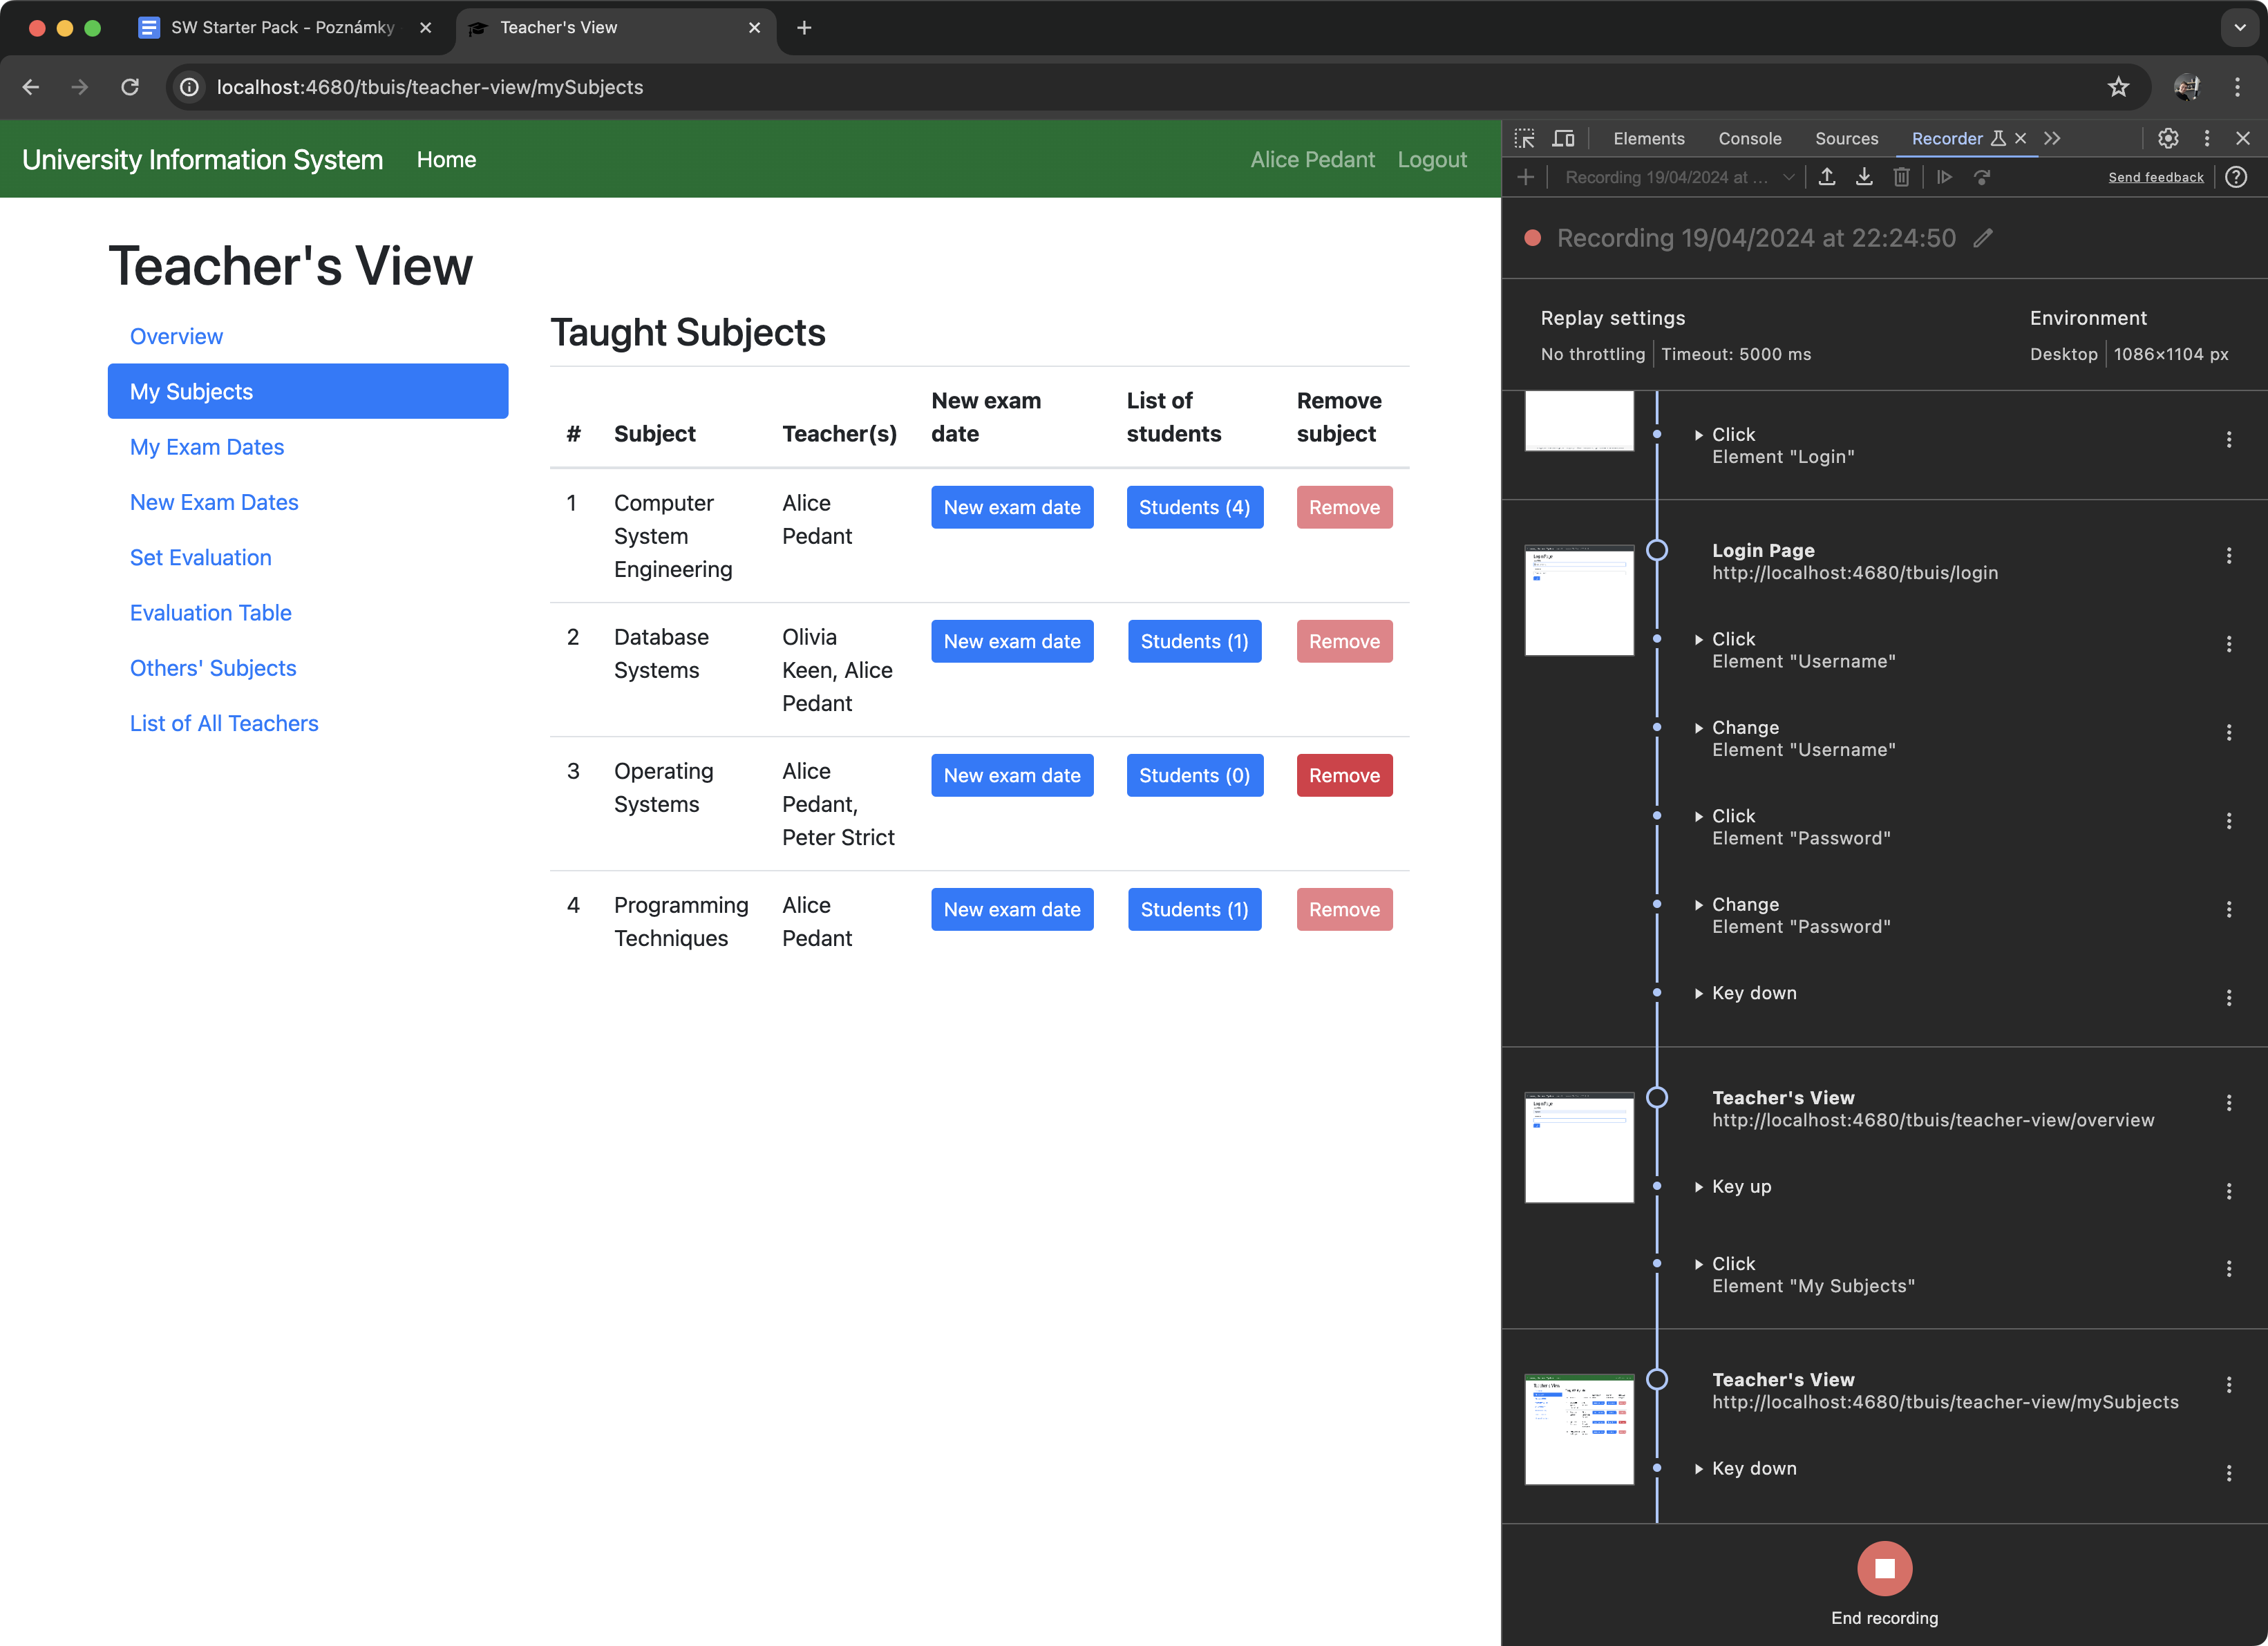
\includegraphics[width=0.8\textwidth]{pic/recording.png}
        \centering
        \caption{Nahrávání scénáře za pomocí nástroje v Google Chrome}
        \label{fig:chrome_recording}
    \end{figure}

    \newpage
    \setuxprompt{milan}{dp/program/input}
    \begin{console}{Ukázková struktura input složky \label{con:input}} 
`\uxprompt`ls -l
milan    448 Apr 21 20:52 ..
milan   3815 Mar 27 20:24 rec-spec-1-student.json
milan   3820 Mar 27 20:28 rec-spec-1-teacher.json
milan   6043 Mar 30 19:42 recording-spec-4-student.json
milan  10635 Mar 31 09:18 recording-spec-4-teacher.json
milan   1370 Apr 21 20:52 spec-1.txt
milan   1328 Mar 31 09:28 spec-4.txt
    \end{console}

    \section{Výběr požadavků}

        \subsection{Vytvoření nového testu} \label{sec:test_creation}

            Primárním programem celé práce je soubor \verb|test.py|, který se nalézá v kořenové složce programu (\verb|/program|) a má konrétně 3 pracovní režimy:
            \begin{enumerate}
                \item Vyvtvoření šablony pro test
                \item Vygenerování testu dle šablony
                \item Spuštění sady testů
            \end{enumerate}
            Právě první režim je v současném kroce důležitý. Jednotlivé režimy programu jsou spuštěny za pomocí argumentů (argumenty jednotlivých režimů ukázané ve výpisu \ref{con:modes}). V případě \textit{vytvoření} nového testu se za argument přidává název šalony testu. Tento název musí být unikání a využívá se později ve zbytku programu jakožto identifikátor daného testu. Po potvrzení příkazu se ve vstupní složce vytvoří nová šablona pro test se zvoleným názvem a příponou \verb|.txt|. Tuto šablonu může uživatel může dále upravit. Celý příkaz je ukázaný ve výpisu \ref{con:new}. Vytvořenou šablonu uživatel zobrazí a upraví v \textit{textovém editoru}.

            \vfill

            \begin{console}{Hlavní režimy programu \label{con:modes}}
`\uxprompt`python3 test.py -n   #Nový test
`\uxprompt`python3 test.py -i   #Generování
`\uxprompt`python3 test.py -r   #Spuštění testů
            \end{console}

            \begin{console}{Vytvoření nového testu (šablony) \label{con:new}}
`\uxprompt`python3 test.py -n specficication-1
            \end{console}

                \begin{code}{text}{Vzor pro vyplnění šablony testu \label{lst:template}}
Write Robot Framework scanario. Open page like in this JSON recording and then when you execute all the steps in the recording, do this:

- //TODO


                \end{code}

                \begin{code}{text}{Vyplněná šablona testu pro specifikaci 18 \label{lst:spec18}}
Write Robot Framework scanario. Open page like in this JSON recording and then when you execute all the steps in the recording, do this:

- Check if there are these names present on the page: Julia Easyrider, Olivia Keen, John Lazy, Alice Pedant, Thomas Scatterbrained, Peter Strict
- Check if element with path //*[@id="tea.listOfAllTeachers.table.teacherRow-0"]/td[3] has text matching "Numerical Methods"
- Check if element with path //*[@id="tea.listOfAllTeachers.table.teacherRow-1"]/td[3] has text matching "Database Systems, Fundamentals of Computer Networks, Introduction to Algorithms, Mobile Applications, Web Programming"
- Check if element with path //*[@id="tea.listOfAllTeachers.table.teacherRow-2"]/td[3] should not contain text
- Check if element with path //*[@id="tea.listOfAllTeachers.table.teacherRow-3"]/td[3] has text matching "Computer System Engineering, Database Systems, Operating Systems, Programming Techniques"
- Check if element with path //*[@id="tea.listOfAllTeachers.table.teacherRow-4"]/td[3] has text matching "Computation Structures"
- Check if element with path //*[@id="tea.listOfAllTeachers.table.teacherRow-5"]/td[3] has text matching "Operating Systems, Programming in Java, Software Engineering, Software Quality Assurance"


                \end{code}

                \subsection{Vyplnění požadavků}

            Do šablony je vložen základní prompt společně s požadavky, které uživatel může vyplnit (viz ukázka \ref{lst:template}). Pod požadavky je defaultně vložena nahrávka \verb|recording.json|. Tuto hodnotu nahradí uživatel za název souboru vložené nahrávky. Formát šablony jakožto vstupu pro prompt testu byl zvolen pro jednodušší parametrizaci. Šablona využívá jazyk \emph{Jinja2}. V rámci vytvořených šablon v této práci byly tyto parametrizační vlastnosti využity například pro vytvoření pohledu \textit{studenta} a \textit{učitele}. Místo, které je v šabloně označeno jako \verb|\\TODO| slouží pro napsání požadavků testu. Od uživatele se čeká, že tyto požadavky vypíše v odrážkách, čemuž odpovídá i formát \emph{promptu}. Ukázka vyplněných požadavků pro konkrétní test je součástí výpisu \ref{lst:spec18}, který ukazuje vypsané vlastnosti pro specifikaci 18, jak bylo popsáno v sekci \ref{sec:scenarios}.


    \section{Dotazování LLM}

        \subsection{Modely a jejich spuštění}
            %Co za modely bylo zvoleno, jejich druhy, atd.
            
            Jak již bylo řečeno v kapitole \ref{sec:research}, velké jazykové modely existují jak v prorietární formě, které jsou dostupné pouze přes API poskytovatele nebo webové rozhraní, ale také se dají najít modely dostupné v \textit{public} či \textit{open source} formě dále referovány jako \emph{otevřené} modely). V rámci tohoto projektu byly využity obě varianty, tedy \emph{proprietární} modely srkze API poskytovatele a otevřené lokálně nebo také srze API u některého z poskytovatelů a to z důvodu vysokých hardwarových nároků některých modelů.Konkrétní seznam použitých modelů v práci včetně typu přístupu k nim lze nalézt v tabulce \ref{tab:used_models}. Pro dotazování vzdálených modelů využívá většina koncových bodů API od OpenAI, tedy jsou kompatibilní s jejich knihovnou pro různé jazyky. Některé společnosti však pro své modely využívají vlastní definici API, mezi ně se řadí například \textit{Anthropic} nebo \textit{Google}. V projektu tedy využíváme pro veškteré kompatibilní modely (resp. jejich běhová prostředí) knihovnu pro OpenAI API, se kterým jsou kompatibilní, a pro zbytek jejich vlastní knihovny.

            \begin{table}
                \catcode`\-=12
                \begin{tabular}{|c|c|c|c|}
                    \hline
                    \textbf{Tvůrce} & \textbf{Model} & \textbf{Použitá verze} & \textbf{Runtime} \\
                    \hline
                    \multirow{3}{*}{OpenAI} & GPT-4 & gpt-4-32k & \multirow{3}{*}{API} \\
                    \cline{2-3} 
                    & GPT-4 Turbo & gpt-4-turbo-2024-04-09 &  \\
                    \cline{2-3} 
                    & GPT-3 Turbo & gpt-3-turbo-0125 &  \\
                    \hline
                    \multirow{2}{*}{Mistral} & Mistral v0.2 7B & TBD & Lokální \\
                    \cline{2-4} 
                     & Mistral Large & mistral-large-2402 & API \textit{La Plateforme} \\
                    \hline
                    Anthropic & Claude 3 Opus & claude-3-opus-20240229 & API \\
                    \hline
                    Meta & Codellama & TBD & Lokální \\
                    \hline
                    Google & Gemini 1.5 Pro & gemini-1.5-pro-preview-0409 & API \textit{Google Cloud} \\
                    \hline
                    % TODO Dopsat modely informace
                \end{tabular}
                \centering
                \caption{Použité LLM modely}
                \label{tab:used_models}
            \end{table}

            \subsubsection{Prostředí pro lokální modely} \label{sec:local_env}

            Pro \emph{lokální} modely a jejich spuštění byl využit software \textit{LM Studio}, který je postaven nad \textit{C++} knihovnou \verb|llama.cpp|. Ta umožňuje jednoduché spuštění \Gls{llm} modelů ve formátu \acrfull{gguf}. Jedná se o \textit{binární} formát souborů určený pro rychlé načítání a ukládání modelů využíváných pro účely interferenčních úloh. Jeho návrh umožňuje snadnou úpravu při zachování zpětné kompatibility. \cite{ggerganov_gguf} \cite{huggingface_gguf} Modely mohou být vyvíjené za pomoci různých frameworků (např. \textit{PyTorch}) a poté převedeny do \acrshort{gguf} formátu pro použití v rámci \acrshort{ggml} knihovny, která umožňuje efektivní spuštění modelů na CPU a GPU. Knihovna také umožňuje \emph{kvantizaci}, tedy techniku využívanou ke snížení paměťových nároků \acrshort{ml} úloh. Zahrnuje reprezentaci vah a aktivací za pomoci datakových typů s nižší přesností (např. \textit{int8}) oproti obvyklým 32 bitovým číslům (např. \textit{float32}), ve kterých bývají reprezentována originální data modelu. Jejím cílem je snížit počet bitů, což vede k nižší velikosti modelu a to k nižším HW nárokům a s tím spojených vlastností (\textit{snížená energetická spotřeba, nižší latence, ...}). Kvantizace má však i nežádoucí dopady a to \textit{ztrátu přesnosti} nebo případně \textit{výkonu} modelu. \cite{huggingface_quantization} \Acrshort{gguf} tedy tvoří jednotný formát, ve kterém se spousta otevřených \Gls{llm} modelů (případně jejich konverzí) distribuuje. Jednou z platforem pro jejich distribuci je například \href{https://huggingface.co}{HuggingFace}.

            % TODO obr LM Studia

            \textit{LM Studio} umožňuje spuštění právě modelů ve formátu \acrshort{gguf}, včetně jejich stažení z repozitářů a funkcemi s tím spojených (například \textit{vypsání seznamu kvantizací, spojení rozdělených modelů, atd.}). Jeho primární funkcí je spouštět lokální \Gls{llm} modely jako \textit{chat} nebo \textit{lokální server} nabízející API kompatibilní s definicí dle OpenAI. Pro každý druh modelů (jako \textit{Llama, Mistral, Command R, ...}) také obsahuje předdefinované nastavení, které si uživatel může upravit. Mezi tímto nastavením jsou hyperparametry jako \textit{\gls{temperature}, Min P, Top P, délka \gls{context}u, maximálního počtu vygenerovaných \gls{token}ů a dalších}. Mimo toho obsahuje i nastavení pro hardware jako \textit{počet vláken CPU, počet GPU vrstev, GPU framework} a podobně. \textit{Vrstvou} je zde myšlena vrstva neutronů, která provádí určit výpočty a zpracování vstupních dat. Vrstvy mohou být ku příkladu \textit{vstupní, skryté, výstupní}. Klíčovou vlastností nastavitelnou v rámci runtimu tohoto softwaru je možnost nastavit chování \gls{context}ového okna. Mezi možnosti se řadí: 
            \begin{enumerate}
                \item \textit{Klouzavé okno} - Model si pamatuje posledních \(x\) tokenů z konverzace, které využívá ke generování výstupu a predikci.
                \item \textit{Začátek a konec} - Model si pamatuje první prompt (případně i systémový) a zbylé tokeny na konci konverzace.
                \item \textit{Zastavení} - Při dosažení počtu tokenů v rámci konverzace rovnající se \(x\), je generování odpovědi zastaveno.
            \end{enumerate}
            Proměnnou \(x\) je zde myšlena celková délka kontextu, kterou \textit{model} nebo \textit{runtime} podporuje. V případě \textit{runtimu} v rámci \textit{LM Studio} (resp. \verb|llama.cpp|) může uživatel délku kontextu zvolit až do délky \(16 384\) \gls{token}ů. Pokud však tato délka bude větší, jak podporovaný kontext samotným modelem, délka kontextu, který model má v paměti, bude dán hodnotou z modelu. Například modely vycházející z architektury \textit{Llama-2} disponují kontextem \(4096\) \gls{token}ů, jak bylo diskutováno v sekci \ref{sec:research_models}. Pokud tedy runtime bude nastaven s větším kontextovým oknem, bude rozhodující právě tato hodnota modelu.
            
            Pro spuštěnou instanci modelu lze také nastavit \textit{systémový prompt}. Jedná se o první zprávu, která se modelu předává a měla by obsahovat pokyny pro model definující jeho chování, roli a další relevatní informace, které mohou zlepšit přesnost jeho výsledků nebo mu umožnit lépe pochopit kontext. Tento prompt je běžně vložen pouze na začátku konerzace a poté uložen do paměti modelu. Ukázku takového systémového promptu lze vidět ve výpisu \ref{lst:system_prompt_example}. Tento konkrétní příklad pochází právě ze softwaru \textit{LM Studio}.

            \begin{code}{text}{Příklad systémového promptu \label{lst:system_prompt_example}}
You're an intelligent programming assistant. Output code only, no text around.
            \end{code}

            \subsubsection{Testovací sestava a nastavení}

            \begin{table}
                \begin{tabular}{|c|c|}
                    \hline
                    \textbf{Typ} & \textbf{Komponenta} \\
                    \hline
                    CPU & AMD Ryzen 8700F \\
                    \hline
                    Základní deska & Asus B650-PLUS TUF \\
                    \hline
                    CPU Chlazení & BOX \\
                    \hline
                    RAM & Kingston FURY Renegade DDR5 64GB 6400 MHz (4x16GB) \\
                    \hline
                    VGA & Radeon RX 7900 XT 20GB Asus TUF \\
                    \hline
                    PSU & ADATA XPG CYBERCORE 1300W \\
                    \hline
                    Case & BeQuiet! Dark Base Pro 901 \\
                    \hline
                \end{tabular}
                \centering
                \caption{Seznam komponent testovací PC sestavy}
                \label{tab:pc_components}
            \end{table}

            Pro spouštění lokálních modelů byla využita PC sestava, jejíž komponenty jsou popsané v tabulce \ref{tab:pc_components}. Runtime programu \textit{LM Studio}, popsaného v minulé sekci, byl nastaven, aby využíval \(12\) z \(16\) dostupných CPU vláken. GPU akcelerace fungovala v režimu \textit{OpenCL}. Počet GPU vrstev se však liší model od modelu. Pro správnou funkčnost je potřeba udržet celý model v paměti RAM, tedy v případě naší sestavy jsme mohli pracovat s modely pouze cca do 60GB, s tím, že do VRAM grafické karty lze nahrát pouze vrstvy o celkové velikosti přibližně 20GB. Na GPU tedy byl akcelerován jen takový počet vrtev, který z jejich celkového počtu odpovídal této velikosti. Délka \textit{kontextového okna} byla nastavena na \(8 192\) \gls{token}ů, avšak pro některé modely je tato délka zkrácena samotným modelem (viz sekce \ref{sec:local_env}). Jednotlivé hyperparametry byly poté nastaveny jako:
            \begin{enumerate}
                \item \textbf{\gls{temperature}}: \(0.7\)
                \item \textbf{Top P}: \(1\)
                \item \textbf{Maximum vygenerovaných tokenů}: \(3000\)
                \item \textbf{režim kontextového okna}: klouzavé okno
            \end{enumerate}
            Zbytek \emph{hyperparametrů} zůstal na defaultních hodnotách daného modelu, který byl testovaný. Toto nastavení bylo využito jak pro \textit{lokální} modely tak pro \textit{API} dotazy na poskytovatele proprietáních či jiných vzdáleně spuštěných modelů. Použité hodnoty těchto parametrů vycházejí z prvotních testovacích experimentů, kdy se osvědčili jako vhodné pro generování jednotkových testů, protože by měli zaručovat \textit{nižší determiničnost} výsledku a jeho \textit{vyšší přesnost}.

        \subsection{Dotazy} \label{sec:llm_requests}
        Samotné vygenerování testů za pomoci dotazování \Gls{llm} je řešeno skrze \textit{generující} režim programu, jako je ukázáno ve výpisu \ref{con:modes}. Tento režim jako argument vyžaduje \textit{název šablony}, která funguje jako \textit{prompt} pro model a byla vytvořena v předchozím kroku (viz sekce \ref{sec:test_creation}). Tento režim poporuje i více nepovinných argumentů jako:
        \begin{itemize}
            \item \verb|count| - Počet variací testů, které se mají vygenerovat. Celé číslo. Defaultní hodnota \(1\).
            \item \verb|manual| - Zkopírovat prompt do schránky pro manuální vložení do rozhraní modelu. Vlajka. Vhodné pro debug.
            \item \verb|cmd| - Vypsat prompt do standardního výstupu. Vlajka.
            \item \verb|compress| - Vlajka vyjadřující použití promptové komprese.
        \end{itemize}

        Mimo argumentů je \textit{generování testů} také konfigurováno \textit{proměnnými prostředí}, které pokud nejsou definovány, program se snaží načíst soubor \verb|.env| (pokud je přítomný), který tyto proměnné obsahuje. Konfigurace generování za pomocí těchto proměnných byla zvolena, protože se většinou nepřidávají do \Acrshort{vcs} nebo je jejich přidání ošetřeno, protože obsahují citlivá data, která by měla zůstat pouze na stroji uživatele. Mezi základní proměnné prostřední patří:
        \begin{itemize}
            \item \verb|API_URL| - Adresa URL, na kterou program dělá API dotazy.
            \item \verb|API_KEY| - Klíč pro přístup ke vzdálenému API (pro lokální modely stačí zadat libovolnou hodnotu nebo nedefinovat).
            \item \verb|API_MODEL| - Název modelu, na kterém programu bude v rámci API požadovat vygenerování výstupu (hodnota dána dokumentací daného API).
            \item \verb|MAX_TOKENS| - Maximální počet tokenů, které má model vygenerovat. V závislosti na dokumentaci API je potřeba nastavit hodnotu v určiném rozsahu.
        \end{itemize}
        Mimo parametrů pro generování může \verb|.env| soubor obsahovat i další parametry (resp. proměnné) určené pro jiné operace programu. Ukázková podoba tohoto souboru je zobrazena ve výpisu \ref{lst:dot_env}. Soubor je umístěn v kořenové složce programu.

        Ukázkové volání programu v režimu generace testů lze vidět v ukázce \ref{con:generation}. Program je schopen vygenerovat pro jeden test více variant na bázi stejného promptu (vytváření nových dotazů na \Gls{llm}). Detailní popis algoritmu je nastíněn v obrázku \ref{fig:llm_query_algo}. \textit{Šablona}, kterou uživatel vytvořil je použita pro \emph{render} finálního promptu za pomocí šablonovacího jazyka \textit{Jinja}. Tato metoda byla zvolena z důvodu \textit{jednoduché a předhledné modifikace} vstupů (zde nazvaých jako \textit{šablon} nebo \textit{uživatelských specifikací}), \textit{možnosti nezávislého vložení nahrávky} a také především případné \textit{parametrizace} vstupu, díky které by mohla jít měnit \textit{uživatelská jména}, \textit{názvy prvků} a další možné údaje v šabloně vhodné pro parametrizaci. 

        \begin{figure}
            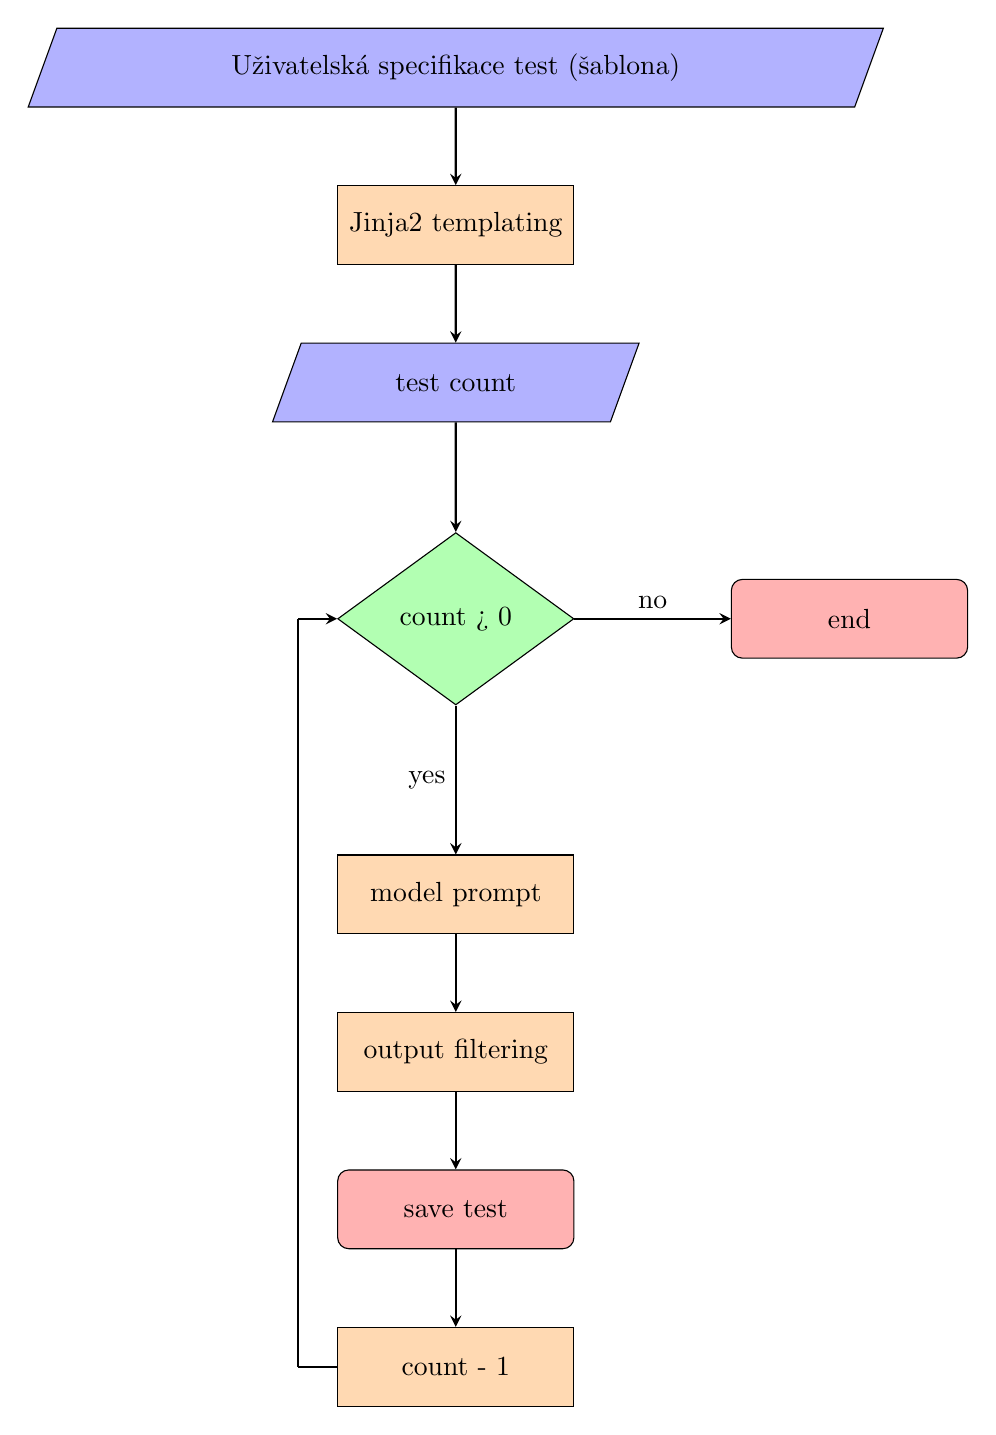
\begin{tikzpicture}[node distance=2cm]
                \node (start) [io] {Uživatelská specifikace test (šablona)};
                \node (in1) [process, below of=start] {Jinja2 templating};
                \node (in2) [io, below of=in1] {test count};
                \node (dec1) [decision, below of=in2, yshift=-1cm] {count > 0};
                \node (pro1) [process, below of=dec1, yshift=-1.5cm] {model prompt};
                \node (pro2) [process, below of=pro1] {output filtering};
                \node (out1) [startstop, below of=pro2] {save test};
                \node (procCount) [process, below of=out1] {count - 1};
                \node (stop) [startstop, right of=dec1, xshift=3cm] {end};
                \coordinate [left of=procCount] (lc);
                \coordinate [left of=dec1] (lif);

                \draw [arrow] (start) -- (in1);
                \draw [arrow] (in1) -- (in2);
                \draw [arrow] (in2) -- (dec1);
                \draw [arrow] (dec1) -- node[anchor=east] {yes} (pro1);
                \draw [arrow] (pro1) -- (pro2);
                \draw [arrow] (pro2) -- (out1);
                \draw [arrow] (out1) -- (procCount);
                \draw [arrow] (dec1) -- node[anchor=south] {no} (stop);
                \draw [arrow] (procCount) -- (lc) (lc) -- (lif) (lif) -- (dec1);
            \end{tikzpicture}
            \centering
            \caption{Zjednodušené schema algoritmu pro dotazování jazykového modelu při generování testu.}
            \label{fig:llm_query_algo}
        \end{figure}

        \setuxprompt{milan}{dp/program}
        \begin{console}{Ukázka volání generace testu dle šablony \label{con:generation}}
`\uxprompt`python3 test.py -i spec-4 --count 10
        \end{console}

        Finální podoba promptu je poté skrze \textit{konektor} pro příslušné \Gls{llm} (například zmíněná \textit{OpenAI} knihovna, \textit{HTTP} dotaz či jiný druh konektoru) předána jako dotaz modelu. Společně s ním je i modelům předán v rámci těchto konektorů i \textit{systémový prompt}. V případě, že se je aktivní vstupní příznak programu \verb|--manual|, systémový prompt se přidá před vyrenderovaný prompt a tento spojený text je zkopírován do \textit{schránky}. Program načítá systémový prompt ze souboru \verb|templates/system.txt|. Jeho znění (viz výpis \ref{lst:system_prompt_used}) vychází poažadavků a nedostatků, které byli při testovacím generování zpozorovány.

        \begin{code}{text}{Použitý systémový prompt \label{lst:system_prompt_used}}
You're an intelligent programming assistant. You write Robot Framework scenarios and scripts using the Selenium Library. Insert delays between steps. Output code only, no text around. Use Chrome as browser. Locate elements using XPath. Close browser between scenarios.
        \end{code}

        \begin{code}{shell}{Ukázka ".env" souboru \label{lst:dot_env}}
API_URL="https://api.mistral.ai/v1"
API_KEY="Zca6nB87qmijn4"
API_MODEL="mistral-large-latest"

MAX_TOKENS=3000
DEVICE="mps"
        \end{code}

        I přes důraz na nutnost pouze \textit{programového} výstupu v rámci systémového promptu, mají modely tendeci tuto podmínku ignorovat a generovat text okolo kódu. Protože jsou modely naučené tak, aby jejich výstup byl text v \textbf{Markdown} formátu, obsahují i značky se začátkem kódového bloku a značením jazyka, ale také prvky jako odrážky, apod. Tyto prvky se pak objevují i ve výstupech, kde je požadován pouze \textit{čistý text} (jako například v ukázce \ref{lst:text_around}). V našem případě je toto chování nevhodné, protože vyžadujeme na výstupu pouze \textit{kód testu}. Díky struktuře \textit{Markdown} formátování však lze lze kód z tohoto výstupu jednoduše vyparsovat. Toto parsování má právě na starosti funkce \textit{filtrování výstupu} ve schematu \ref{fig:llm_query_algo}. V rámci programu byla implementována tak, že ze vstupního textu vyjme kód v prvním nalezeném kódovém bloku, označeného pomocí znaků \verb|```|. Pokud blok nenajde, vrátí původní text bez změny (předpokládá, že model se držel systémového promptu). V případě více kódových bloků přítomných ve výstupu, kdy požadovaný kód nebude v prvním z bloků, dojde k nesprávnému parsování, avšak jedná se o očekávaný případ, protože detekce správného kódu je \texti{netriviální} a zároveň \textit{subjektivní} problematika.

        \begin{code}{robotframework}{Výstup modelu s nadbytečným textem. \label{lst:text_around}}
Here's a Robot Framework scenario that follows the recorded JSON steps for interacting with the web page, and then performs the checks as specified:

```robotframework
*** Settings ***
Library           SeleniumLibrary

*** Variables ***
${URL}            http://localhost:4680/tbuis/index.jsp
${USERNAME}       lazy
${PASSWORD}       pass
${BROWSER}        Chrome

*** Test Cases ***
Open and Verify Webpage Content
...
```

In this Robot Framework script, I've incorporated commands that:
- Open the specified page and set the viewport size.
- Perform the login process using the provided username and password.
- Navigate to the "List of All Teachers" section.
- Check for the presence of specified names on the page.
- Validate the text content of specific table cells related to the teachers' courses.
Adjust the locators (xpath) as necessary to match the exact structure and identifiers used in your application's HTML.
        \end{code}

        Vyfiltrovaný výstupní text modelu je poté zapsán do souboru ve výstupní složce nazvané \verb|generated|, nacházející se v kořenové složce programu. Test je uložen s názvem ve formátu \verb|{nazev-vstupu}-{cislo-varianty}.robot| jakožto \textit{RobotFramework} soubor. První část tohoto názvu souhlasí s názvem \textit{promptové šablony}, pro kterou uživatel vytváří testy. Druhá část poté čísluje vygenerované varianty. Pokud již ve výstupní složce existuje vygenerovaný test pro danou specifikaci, program nové variantě přiřadí číslo o \(1\) vyšší, tedy pokračuje v číselné řadě. Názvy vygenerovaných testů jsou postupně vypisovány do konzole. Od uživatele je očekáváno, že vygenerované testy ve výstupní složce zkontroluje a ověří, že obsahují validní (\textit{např. obsahuje text, připomínající RobotFramework test}). Je zde totiž stále možnost, že model nevygenerovat žádný kód a vypsat pouze text nebo \textit{filtrace} neproběhla validně. Tento krok by v ideálním případě bylo možné automatizovat za pomocí \textit{analyzátoru} pro \textit{RobotFramework}, který se nachází v rámci \Gls{lsp} pro \textit{RobotFramework} \verb|rebotframework-lsp| nachází. Bohužel však neumí validovat zápis pro knihovnu \verb|SeleniumLibrary|, která je v rámci systémového promptu vyžadována a očekávána, že bude přítomná ve vygenerovaném testu.

        %TODO možná pak někde vysvětlit, co to ta SeleniumLibrary je a jak vlastně funguje testování v Robot Frameworku

\chapter{Spuštění testů}

    \section{Spuštění testovaného programu a jeho orchestrace}

    %TODO tady nějaké citace
    Testovaný program \textit{TbUIS} (popsaný v sekci \ref{sec:test_program}) je distribuován jakožto \verb|.WAR| soubory, tedy komprimovaný webový archiv jazyka Java, spustitelný jakožto \gls{servlet}. Z dokumentace projektu a předchozích diplomových prací vyplývá, že pro nasatení je určený aplikační server \textit{Tomcat} verze \(7\) až \(9\). S vyššími verzemi není aplikace kompatibilní. Každá varianta aplikace (\textit{poruchové klony}) je distribuována jako samostatný \textit{WAR} soubor. Pro spuštění konkrétní varinaty a spuštění vygenerovaných testů na této variantě bylo nutné vytvořit \textit{automatizované nasazení} aplikace \textit{TbUIS}. Pro nasazení je nutné brát v úvahu nejen samotnou webovou aplikaci, ale i její závislost, kterou je \textit{databáze} MySQL (resp. MariaDB), která musí být inicializována dodaným skriptem.

    \subsection{Vytvoření kompozice} \label{sec:composition}
    Pro účely \textit{automatizovaného nasazení} byla zvolena technologie \textit{Docker}, tedy \textit{kontejnerové} řešení s možností vytvářet obrazy a kompozice. Právě kompozice je vhodným nástrojem pro jednoduché \textit{lokální} nasazení aplikace \textit{TbUIS}, protože potřebujeme 2 samostatné kontejnery; první s \textit{aplikačním servervem} a druhý s \textit{databází}.

    Před samotnou integrací je nutné v každé z variant aplikace (\textit{WAR} soubory) změnit \textit{adresu} databáze. Docker kompozice umoňují přidělit jednotlivým kontejnerům názvy, za pomocí kterých lze v rámci interní DNS tyto kontejnery adresovat. V rámci archivů bylo nutné modifikovat adresu v souborech \textit{WEB-INF/classes/META-INF/persistence.xml} a \textit{WEB-INF/classes/applicationContext.xml}. Pro zjednodušení vlastního nasazení jsou modifikované webové archivy součástí repozitáře této práce. Pro kontejner \textit{databáze} byl zvolen název \verb|tbuis-db|. Veškeré potřebné soubory pro spuštění testovaného programu se nachází ve složce \verb|tbuis| v rámci programové složky.

    K vytvoření \textit{kompozice} je potřeba mít také obrazy, ze kterých se budou vytvářet kontejnery. Zatímco pro databázi stačí \textit{MariaDB} kontejner z veřejného repozitáře, tak pro aplikační server je potřeba vytořit vlastní obraz, který bude vycházet z obrazu pro \textit{Tomcat} aplikační server, ale vždy do něj budou nahrána data jiné varianty aplikace. Pro vytoření obrazu byl do složky přidán \textit{Dockerfile} sloužící k jeho sestavení. Obsah tohoto souboru lze vidět v ukázce \ref{lst:dockerfile}. Skript přebírá cestu k \textit{WAR} souboru za pomocí argumentu a ten poté vkládá do obrazu na předem definovanou cestu a s definovaným názvem. V rámci Tomcat kontejneru slouží právě složka \verb|webapps| pro servlety a jejich název udává cestu, které v rámci HTTP dotazů jsou dostupné. Pro zvolený název \verb|tbuis| tedy odpovídá cesta \verb|/tbuis|.

    \begin{code}{dockerfile}{Dockerfile pro sestavení obrazu varianty aplikačního serveru. \label{lst:dockerfile}}
FROM tomcat:9.0
ARG WAR_FILE
COPY ${WAR_FILE} /usr/local/tomcat/webapps/tbuis.war
    \end{code}

    Obraz z \textit{Dockerfile} lze vytvořit samostatně, ale také lze jeho sestavení zavolat při vytváření kompozice. To se provádí nástrojem \textit{Docker Compose}. Defaultní název souboru, který příkaz pro vytváření kompozice \verb|docker-compose up| využívá je \verb|docker-compose.yml|. Takovýto defaultní soubor je vytvořen v podsložce programu \verb|tbuis| (jeho obsah se nachází v ukázce \ref{lst:docker-compose}). Jak přípony souboru vyplývá, jedná se o textový soubor ve formátu \textit{YAML}. V rámci něj definujeme dvojici služeb potřebných pro nasazení aplikace. Službou v kompozici je myšlen kontejner. Při vytváření služby lze definovat i její \textit{proměnné prostředí}, \textit{porty} a jejich předávání, \textit{připojené} složky, \textit{sítě} a další vlastnosti běžně nastavované pro kontejner. Pro \textit{databázi} je potřeba předat port \(3306\), ale také připojit složku s inicializačními skripty (v našem případě dostupná ve stejné složce jako kompoziční soubor). V ní se nachází soubor \verb|init-db.sql|, který obsahuje příkazy pro vytvoření databáze s daným názvem a uživatele, za kterého se aplikační server připojuje. U služby aplikačního serveru je potřeba sestavit obraz. Pro toto sestavení využíváme vytvořený Dockerfile, nacházející se ve stejné složce. Také je potřeba předat argument s cestou pro \textit{WAR} soubor, který bude do serveru nahraný. Pro přístup do webového rozhraní aplikace z venčí kompozice byl zvolen port \(4680\) předaný z defaultního portu \(8080\), který aplikace používá. Tento port bude sloužit vygenerovaným testům pro přístup. V případě potřeby může uživatel tento port změnit dle svých požadavků. Oba kontejnery jsou také připojeny do stejné \textit{virtuální sítě}, který zajišťuje komunikaci mezi nimi. 

    \begin{code}{dockerfile}{Docker Compose soubor pro sestavení kompozice \label{lst:docker-compose}}
version: '3.8'

services: 

  db:
    image: mariadb
    container_name: tbuis-db
    environment: 
      MARIADB_ROOT_PASSWORD: testtest
    ports:
      - "3306:3306"
    volumes: 
      - ./db:/docker-entrypoint-initdb.d/
    networks:
      - tbuis

  tomcat:
    build:
      context: .
      args:
        WAR_FILE: ${WAR_FILE_PATH}
    container_name: tbuis-tomcat
    depends_on:
      - db
    ports:
      - "4680:8080"
    networks:
      - tbuis

networks: 
  tbuis:
    driver: bridge
    \end{code}

    Pro vytvoření a spuštění této kompozice je potřeba zavolat příkaz z ukázky \ref{lst:compose_up_command}, kde příkaz \verb|up| vyjadřuje právě \textit{vytvoření} kompozice. Pro povolení sestavení obrazu v rámci vytváření kompozice, je také potřeba přidat argument \verb|--build|. Aby se kontejnery spustili na pozadí a ne v terminálu, je také vyžadován argument \verb|-d|. Zároveň z důvodu, abychom nástroj \verb|docker-compose| nemuseli volat pouze ze složky, ve které se kompoziční soubor nachází, lze také přidat argument \verb|-f| a hodnotou cesty ke konfiguračnímu souboru. Před příkazem je také vyexportována proměnná prostředí \verb|WAR_FILE_PATH|, která určuje variantu serverletu, který bude nasazen do webové aplikace. Jedná se o cestu relativní vůči \textit{docker compose} souboru. V případě nutnosti \textit{smazat} kompozici, je také možnost zavolat příkaz \verb|docker-compose down| (viz ukázka \ref{lst:compose_down_command}). Protože při vytváření kompozic byli sestaveny i obrazy, které mohou na počítači zbírat nemalé místo, je také k příkazu přidán argument \verb|--rmi all|, který mimo kotejnerů vytvořených kompozicí smaže i nevyužívané obrazy.

    \setuxprompt{milan}{dp/program}
    \begin{console}{Vytvoření Docker kompozice z připravené konfigurace \label{lst:compose_up_command}}
`\uxprompt`WAR_FILE_PATH=./defect-00_free.war docker-compose -f tbuis/docker-compose.yml up -d --build
    \end{console}

    \begin{console}{Smazání Docker kompozice společně s vytvořenými obrazy \label{lst:compose_down_command}}
`\uxprompt`docker-compose -f tbuis/docker-compose.yml down --rmi all
    \end{console}

    \subsection{Orchestrace a automatizace nasazení} \label{sec:orchestration}

    Výše vypsané příkazy automatizují nasazení jedné z variant webové aplikace. Namísto jejich manuálního volání však bude tento úkon provádět orchestrační program \verb|test.py| v režimu \verb|-r| (\textit{run}). Příklad takového volání se nachází v ukázce \ref{lst:run_mode}. Samotná orchestrace spuštění vygenerovaných testů spočívá v tom, že program nasadí jednu z požadovaných variant aplikace, poté postupně spustí jednotlivé testy vyhovující zadanému kritériu v rámci hodnoty pro argument režimu \verb|-r|. Po dokončení všech testů je načtena další z požadovaných verzí aplikace pro nasazení a otestování. Zvolené testy jsou tedy spuštěny na všech vybraných variantách (orchestrace nastíněna v obr. \ref{fig:orchestration}). Po dokončení testování je poté vytvořená kompozice společně se všemi jejími sestavenými a staženými obrazy smazána. K těmto úkonům je využit právě nástroj \textit{Docker} a \textit{Docker Compose}, popsané v sekci \ref{sec:composition}. Mezi jednotlivými testy spouštěnými na jedné z variant aplikace je také potřebna provést \textit{obnovení databáze}, protože některé z testovacích scénářů databázi modifikují (viz tabulky \ref{tab:specs_1} a \ref{tab:specs_2}). Pro toto obnovení nabízí aplikace \textit{HTTP} endpoint nebo tlačítko na úvodní stránce. Pro zjednodušení byl mezi statické soubory přidán RobotFramework scénář, který na toto tlačítko na úvodní stránce klikne.

    \begin{console}{Spuštění orchestračního programu v režimu spouštění testů \label{lst:run_mode}}
`\uxprompt`python3 test.py -r "codellama/spec-*" --name "codellama-runs"
    \end{console}

    %TODO Obrázek orchestrace
    \begin{figure}
        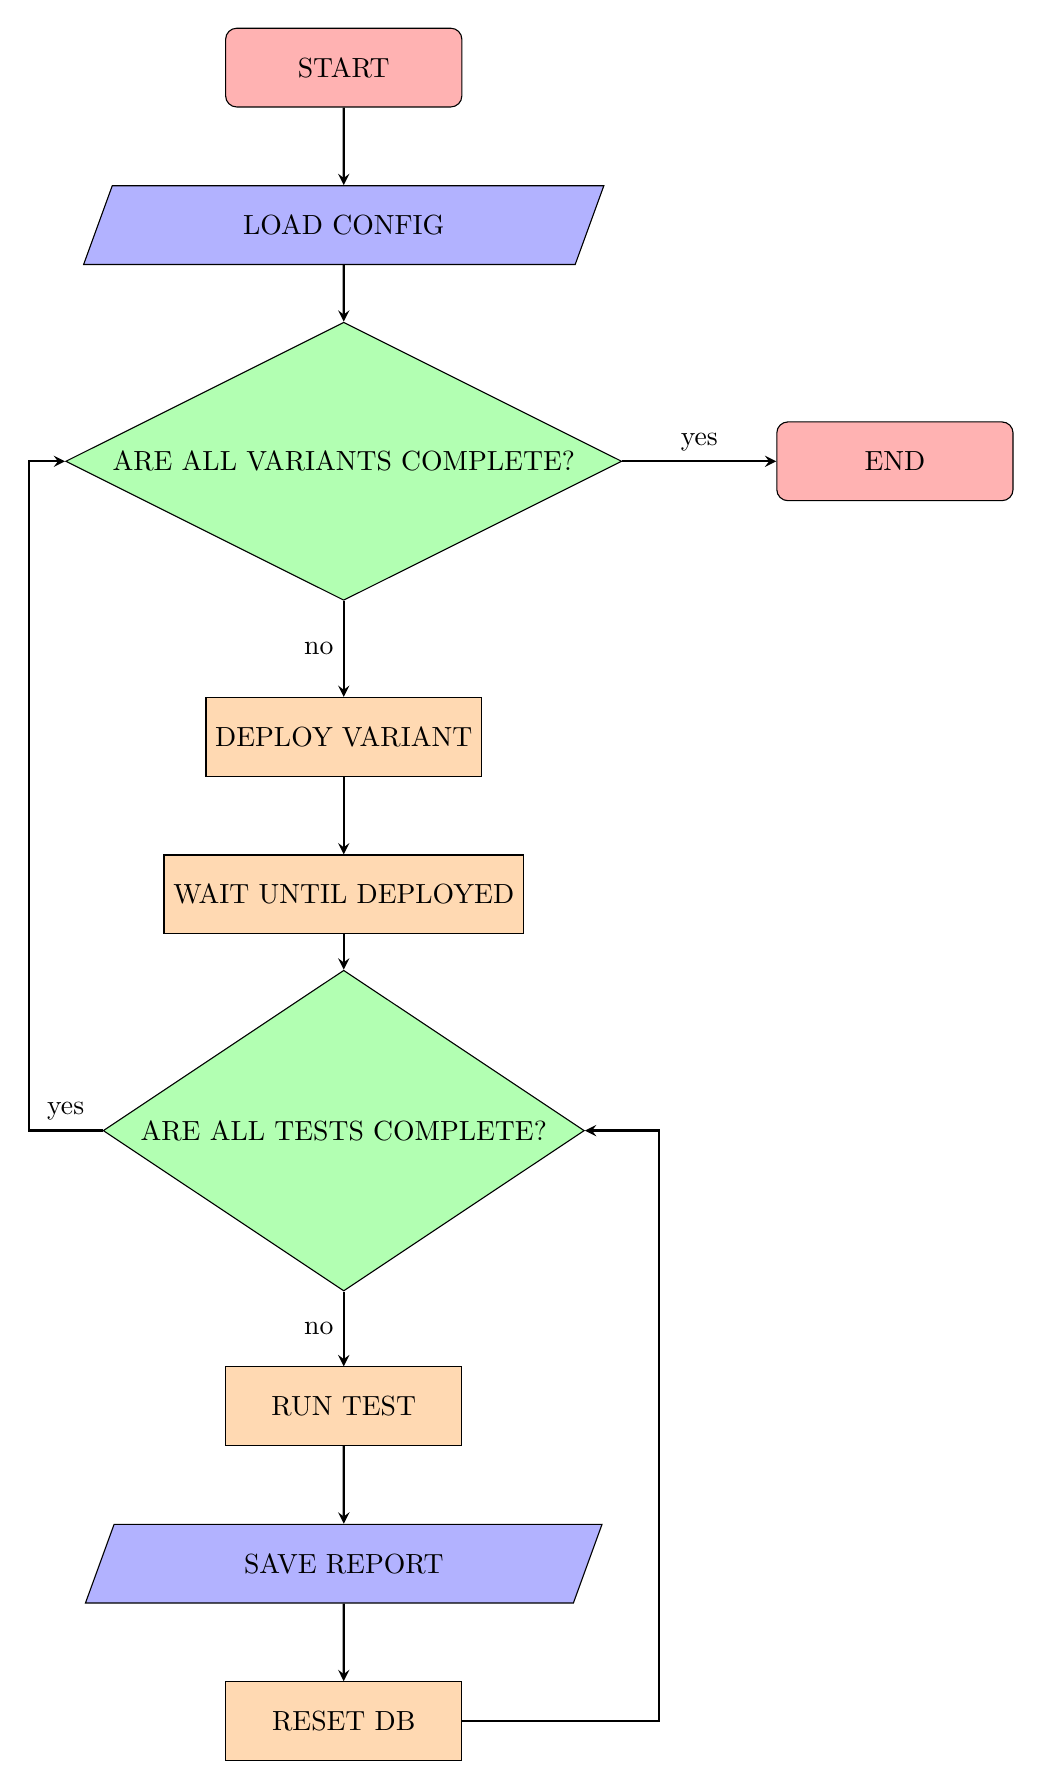
\begin{tikzpicture}[node distance=2cm]
            \node (start) [startstop] {START};
            \node (loadConfig) [io, below of=start] {LOAD CONFIG};
            \node (decision1) [decision, aspect=2, below of=loadConfig, yshift=-1cm] {ARE ALL VARIANTS COMPLETE?};
            \node (end) [startstop, right of=decision1, xshift=5cm] {END};
            \node (deployVariant) [process, below of=decision1, yshift=-1.5cm] {DEPLOY VARIANT};
            \node (waitDeploy) [process, below of=deployVariant] {WAIT UNTIL DEPLOYED};
            \node (decision2) [decision, aspect=1.5, below of=waitDeploy, yshift=-1cm] {ARE ALL TESTS COMPLETE?};
            \node (runTest) [process, below of=decision2, yshift=-1.5cm] {RUN TEST};
            \node (saveReport) [io, below of=runTest] {SAVE REPORT};
            \node (resetDB) [process, below of=saveReport] {RESET DB};
            \coordinate [left of=decision1, xshift=-2cm] (ld1);
            \coordinate [left of=decision2, xshift=-2cm] (ld2);
            \coordinate [right of=resetDB, xshift=2cm] (rdb);
            \coordinate [right of=decision2, xshift=2cm] (rd2);

            \draw [arrow] (start) -- (loadConfig);
            \draw [arrow] (loadConfig) -- (decision1);
            \draw [arrow] (decision1) -- node[anchor=east] {no} (deployVariant);
            \draw [arrow] (deployVariant) -- (waitDeploy);
            \draw [arrow] (waitDeploy) -- (decision2);
            \draw [arrow] (decision2) -- node[anchor=east] {no} (runTest);
            \draw [arrow] (runTest) -- (saveReport);
            \draw [arrow] (saveReport) -- (resetDB);
            \draw [arrow] (decision1.east) -- node[anchor=south] {yes} (end);
            \draw [arrow] (decision2.west) -- node[anchor=south] {yes} (ld2) -- (ld1) -- (decision1.west);
            \draw [arrow] (resetDB) -- (rdb) -- (rd2) -- (decision2.east);
        \end{tikzpicture}
        \centering
        \caption{Znázornění orchestrace spouštění testů}
        \label{fig:orchestration}
    \end{figure}

    Spuštící režim programu nabízí možnost hned několika argumentů a jejich hodnot. Požadovaná hodnota je zde pro \textit{režimový} argument \verb|-r|, která musí obsahovat název nebo vzor názvu testů, které se v rámci složky \textit{generated} mají spustit. Pro přehlednost si uživatel může ve výstupní složce testů rozdělovat vygenerované testy do podsložek, případně držet vhodnou konvenci pro jejich označení. Hodnota pro vzor názvu testů může být jakýkoliv validní \textit{UNIX wildcard} pro označení souborů. Příklad použití takovéto \textit{wildcard} lze vidět v ukázce \ref{lst:run_mode}, kde se spouští testy (resp. soubory) z podsložky \verb|codellama|, které vyhovují vzoru \verb|spec-*|, což znamená všechny soubory začínající řetězcem "spec-"  v této podsložce. Tento přístup pro zvolení cesty a souborů umožňuje nejen právě dělit výstupní složku testů na podsložky, ale také uživateli spustit jen konkrétní vybrané testy. Spuštění pouze omezené množiny testů je ukázáno ve výpisu \ref{lst:run_mode_2}, kde uživatel požaduje spustit testy vyhovující specifikaci \(1\), \(4\) a \(6\) ve všech jejich varintách (značení vygenerovaných testů popsáno v sekci \ref{sec:llm_requests}) ve složce "openai-gpt-4" (tedy například testy vygenerované modelem GPT-4 od OpenAI). Hodnoty pro tento argument je vhodné psát v \emph{uvozovkách}.

    \begin{console}{Alternativní volání režimu spuštění testů \label{lst:run_mode_2}}
`\uxprompt`python3 test.py -r "openai-gpt-4/spec-{1,4,6}-*" --cont_count 2 --name "gpt-4 test runs"
    \end{console}

    Další argumenty pro \textit{spouštěcí} řežim jsou již \emph{nepovinné}, avšak alespoň argument \verb|--name| je doporučený. Pomocí toho argumentu lze nastavit jméno aktuálního běhu testů, pomocí kterého lze poté jednoduše identifikovat s ním související výsledky. Samotné výsledky, jejich ukládání a struktura jsou vysvětleny v následující sekci kapitoly. Pro hodnotu tohoto argumentu je také doporučené využít uvozovky (ukázkové volání jak v příkladu \ref{lst:run_mode} a \ref{lst:run_mode_2}). Pro zkušební běhy testů lze také využít argument \verb|--cont_count|, jehož hodnota omezí počet volaných variant aplikace, dostupných z \textit{konfigurace} (číselná hodnota vyšší než \(0\)).

    Samotný běh aplikace, testů a jejich případného vyhodnocení neovlivňují pouze \emph{argumenty}, ale také komplexnější \emph{konfigurace}, která se nachází v rámci konfiguračního souboru \verb|configuration.py|. Jednotlivé varinaty aplikace, které se budou spouštět v rámci běhu lze zvolit tak, že se názvy jejich \textit{WAR} souborů ze složky \verb|tbuis| přidají do pole \verb|RUN_CONTAINERS| v rámci konfigurace. 

    \begin{code}{python}{Zjednodušená ukázka konfiguračního souboru \label{lst:configuration}}
RUN_CONTAINERS = [
    "defect-00_free.war",
    "defect-02-C0.H0.M0.L1_S_S_03.war",
    "defect-04-C0.H0.M0.L1_S_S_04.war",
    ...
    "defect-26-C1.H0.M0.L0_T_S_01.war",
    "defect-27-C1.H0.M0.L0_U_D_01.war",
    "defect-28-C2.H2.M1.L0_M_CR.war"
]

POSITIVE_FAILS = {
    "1": ["defect-02-C0.H0.M0.L1_S_S_03.war"],
    "4": ["defect-04-C0.H0.M0.L1_S_S_04.war", "defect-19-C0.H1.M0.L0_S_S_10.war", "defect-25-C1.H0.M0.L0_S_S_01.war", "defect-26-C1.H0.M0.L0_T_S_01.war", "defect-28-C2.H2.M1.L0_M_CR.war"],
    "6": ["defect-25-C1.H0.M0.L0_S_S_01.war", "defect-26-C1.H0.M0.L0_T_S_01.war", "defect-28-C2.H2.M1.L0_M_CR.war"],
    ...
}
    \end{code}
    
    \section{Ukládání výsledků}
    Při spuštění testu vyváří \textit{RobotFramework} hned několik výstupních souborů, mezi kterými je i \textit{report} jakožto soubor \verb|output.xml|. V rámci něj se nacházejí veškteré klíčové informace o běhu scénáře. Konkrétně jde o \textit{log} provedených úkonů, \textit{výsledky} jednotlivých testovacích případů a také případné \textit{errory}. Protože tento výstup obsahuje spoustu redundantních informací, je v rámci programu přeparsován a uložen na 2 samostatná místa. Z původního výstupu jsou parsovány hodnoty: \textit{počet úspěšných}, \textit{neúspěšných} a \textit{chybových} testovacích případů pro každý ze spuštěných testovacích scénářů. Pro ten je vždy také vyhodnocen koncový stav (\textit{FAIL, PASS} nebo \textit{ERROR}). Protože \textit{RobotFramework} nerozlišuje mezi testem, který \emph{selhal} a testem, který neměl spustit nebo při jeho běhu došlo k chybě nesouvisející se scénářem, bylo potřena toto rozlišení implementovat na bázi přítomných \textit{errorů} v rámci výstupního souboru. 

    Pro označení výsledku testu (dále také jako \emph{report}) je využito \textit{časové razítko} doby spuštění série testů ve formátu \verb|YYYYMMDDhhmmss| společně s vybraným názvem v rámci argumentu (popsáno v předchozí sekci \ref{sec:orchestration}) oddělěných znakem "-". V případě, že samostatný název běhu testů není uživatelem vybrán, zůstává pro plné označení reportu pouze časové razítko.

    Prvním z míst pro uložení výsledků je textový soubor uložený ve podsložce \verb|reports| v rámci kořenové složky programu. V rámci tohoto souboru jsou vykresleny textové tabulky, vykreslené pro každou nasazenou variantu aplikace (varianty jsou v rámci programu také označovány jako kontejnery, protože odpovídají kontejneru Dockeru). V rámci tabulky jsou pro každý spuštěný test vypsány výsledky jednotlivých sledovaných údajů a koncový výsledek testu. Ukázka tabulky je vyzobrazena na obr. \ref{fig:report_table}. Název tabulky odpovídá právě testovanému kontejneru (resp. varianty testu). Soubor report je pojmenovaný jeho celým názvem, jak bylo popsáno v předchozím odstavci.

    Ačkoliv tabulková reprezentace výsledků v textové podobě je jednoduchá pro uživatele a jeho čtení, tak již není vhodná pro strojové čtení a zpracování, proto jako druhá možnost pro uložení výsledů byla zvolena \textit{SQLite} databáze, resp. soubor \verb|report_db.sqlite| umístěný ve stejné podložce \verb|reports| jako textové reporty. Tento druh formátu byl zvolen z důvodu jeho jednoduchosti a široké podpoře napříč programovacími jazyky. V rámci této databáze je vytvořena tabulka "runs", která obsahuje řádky s hodnotami výsledků jednotlivých testovacích scénářů, podobně jako v případě tabulek textového reportu. Narozdíl od nich se zde pro veškeré údaje využívá jedna tabulka a mezi jednotlivými běhy jde rozlišit primárně dle jejich názvu. Ukázka tabulky je vyzobrazena na obr. \ref{fig:sqlite_report}. V rámci malé lokální databáze je poté možné data efektivně vyhledávat, filtrovat a nadále s nimi pracovat.
   
    \begin{figure}
        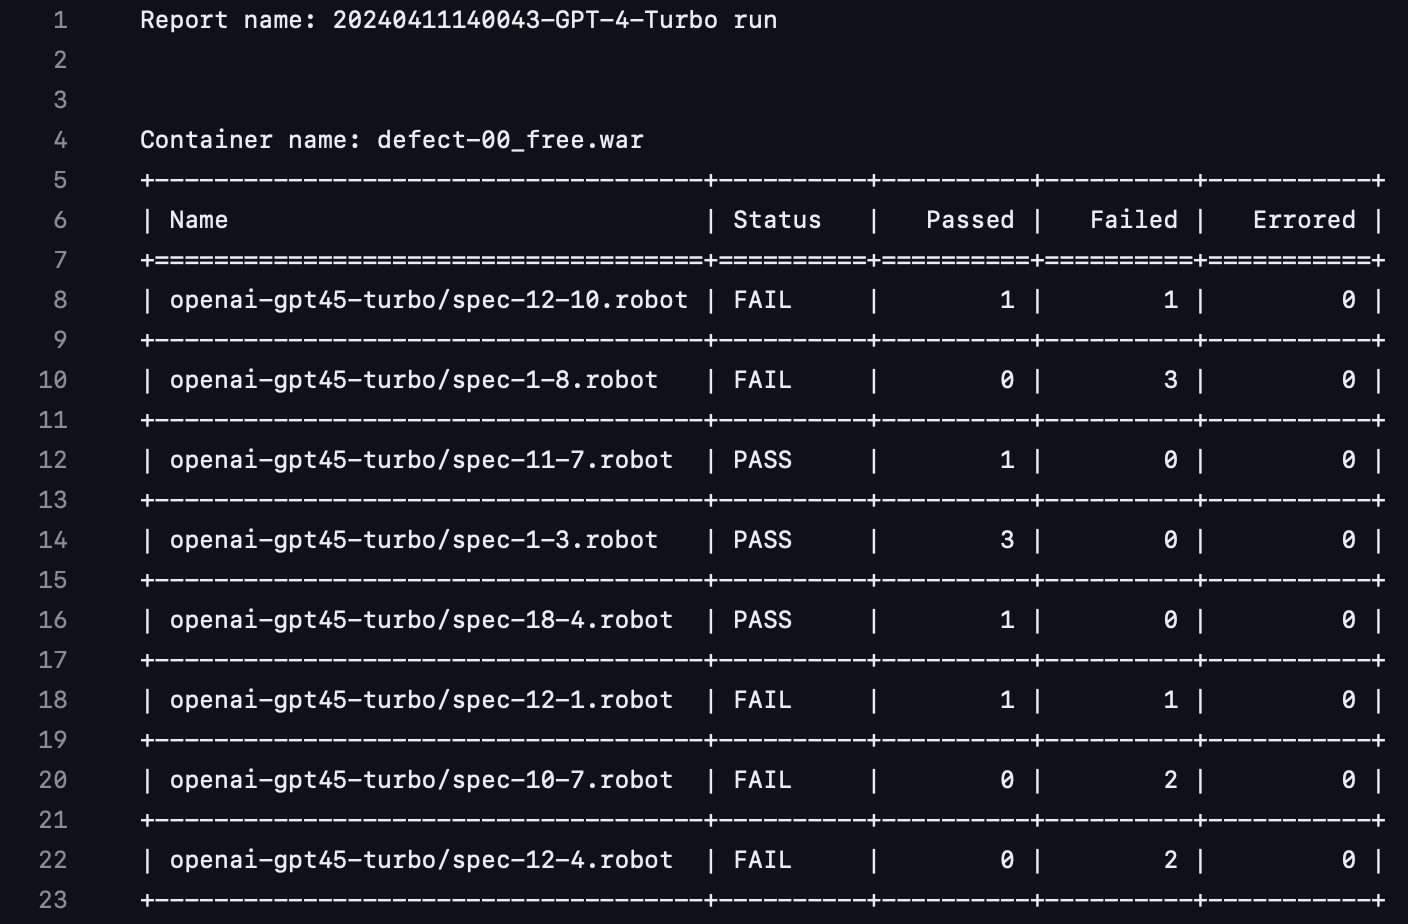
\includegraphics[width=0.8\textwidth]{pic/report_table.png}
        \centering
        \caption{Ukázka textové tabulky výsledků}
        \label{fig:report_table}
    \end{figure}

    \begin{figure}
        %TODO Přidat ukázku ze SQLite db
        \centering
        \caption{Ukázka databázové tabulky výsledků}
        \label{fig:sqlite_report}
    \end{figure}

    %TODO někam pak vypsat prerekvizity pro spuštění programu

\chapter{Vyhodnocení výsledků}

    \section{Parametry pro spuštění} \label{sec:run_parameters}

    Vygenerované testy z kroku \ref{sec:test_generation} (konkrétně scénáře vypsané v tabulkách \ref{tab:specs_1} a \ref{tab:specs_2}) byly v rámci výstupní složky \verb|generated| rozděleny do podsložek s odpovídajícím názvem, ze kterého je patrné, jakým modelem (případně od jaké společnosti) byly vygenerovány. Možnost takového rozdělení byla popsán v sekci \ref{sec:orchestration}. Tyto vygenerové testy, využité k následnému testování poruchových klonů, jsou součástí programového repozitáře projektu. Do konfiguračního souboru byli přidány varianty aplikace dle tabulky \ref{tab:clones} (ukázka konfiguračního souboru ve výpisu \ref{lst:configuration}). Z tabulky scénářů také víme, pro které varianty testovacího programu také můžeme očekávat chybu v daném scénáři. Proto je do konfiguračního souboru přidáno i \textit{mapování}, které každému scénáři (označené pouze číslem) přiřazuje pole názvů \textit{WAR} souborů aplikace, ve kterých je chybovost očekávána. Na bázi tohoto mapování dále vyhodnocovací program určí správnost výsledku testu (tj. v případě očekávaného selhávání jde o správný výsledek). Tento program a použité metody jsou popsány v následující sekci.

    %TODO Asi ukázka ls command výstupní složky
    
    \section{Metodologie vyhodnocení}
        
        \subsection{Vyhodnocovací program}

        Pro vyhodnocení výsledů byl do programové složky vytvořen program \verb|stats.py|, který jako první argument vyžaduje cestu s \verb|.sqlite| výstupnímu reportu hlavního programu v režimu běhu (viz sekce \ref{sec:orchestration}). Tento report si uživatel může libovolně přesouvat v souborovém systému. Reporty vygenerované v rámci tohoto projektu a využité pro hodnocení modelů byli uloženy do podsložky \verb|results| kořenové složky repozitáře. Program má i další argumenty, které jsou jeho klíčovou součástí:
        \begin{itemize}
            \item \verb|-t [nadpis]| - Nastaví nadpis nad tabulkou (název modelu).
            \item \verb|-e [nazev_souboru]| - Vyexportuje soubor do PDF. Hodnotou je název výstupního PDF souboru (s příponou).
        \end{itemize}
        Pro každý test je vyhodnoceno, kolik z jeho vygenerovaných variant pro každou variantu testovacího programu skončilo s \textit{očekávaným výsledkem}. Tím je zde myšleno, že test prošel úspěšně na variantách aplikace, kde se nevyskytuje chyba a je tak očekáván bezchybný průchod, a že test selhal v na takových variantách, kde je definováno specifikací (diskutováno v sekci \ref{sec:run_parameters}), že by selhat měl. Chybový test je vždy považován za \textit{neočekávaný výsledek}. Při takto naivním přístupu by však jako \emph{očekávané} byly označovány i testy (resp. jejich vygenerované varianty) chybující i v případě nasazených variant aplikace bez konkrétní testované chyby (tedy falešná negativa). Z důvodu, aby takové testy nezkreslovali výsledky, bylo přistoupeno ke kroku jejich vyfiltrování a následnému ignorování při vyhodnocování výsledků.

        Pro odhalení falešných negativ budeme využívat předpokladu výsledku na \emph{neporuchové} variantě aplikace, že varianta testu skončí úspěšně. V případě, kdy dojde k jejímu selhání nebo skončí chybou, je taková testová varinta ignorována při vyhodnocení výsledků testů na všech poruchových kontejnerech, protože se předpokládá, že takový test není schopen správně odhadit chybu aplikace, protože by chybový stav hlásil vždy. Počet ignorovaných variant od každého testu je zobrazen ve spodní řádce tabulky výsledků (více v následující sekci \ref{sec:plot_legend}).

        %TODO Volání stats programu

        \subsection{Legenda grafů} \label{sec:plot_legend}

        %TODO Kam jsem uložil výsledky

    %TODO Někam pak taky ověření, že výběr true negatives je správný - asi sem

    \section{Výsledky pro jednotlivé modely}
    
        \subsection{OpenAI}

            \begin{figure}
                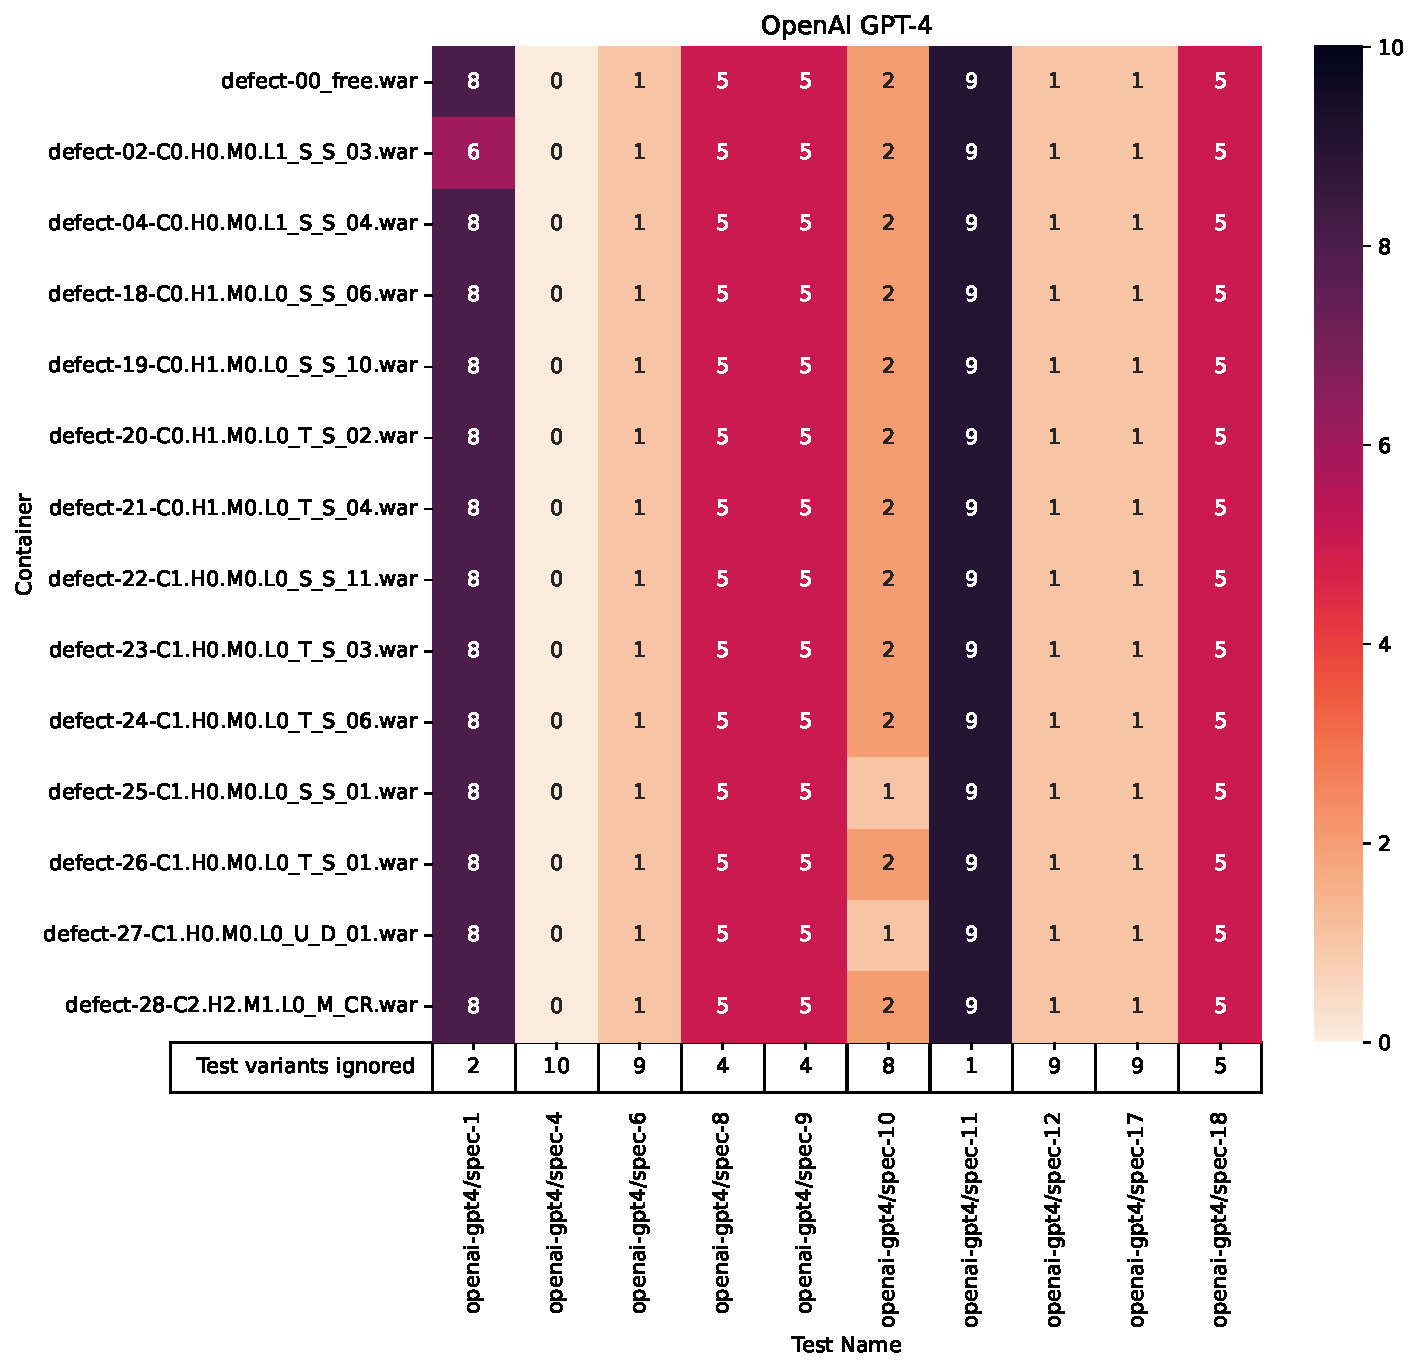
\includegraphics[width=\textwidth]{pic/gpt-4-results.pdf}
                \caption{Výsledky pro model GPT-4}
                \label{fig:res:gpt-4}
            \end{figure}

            \begin{figure}
                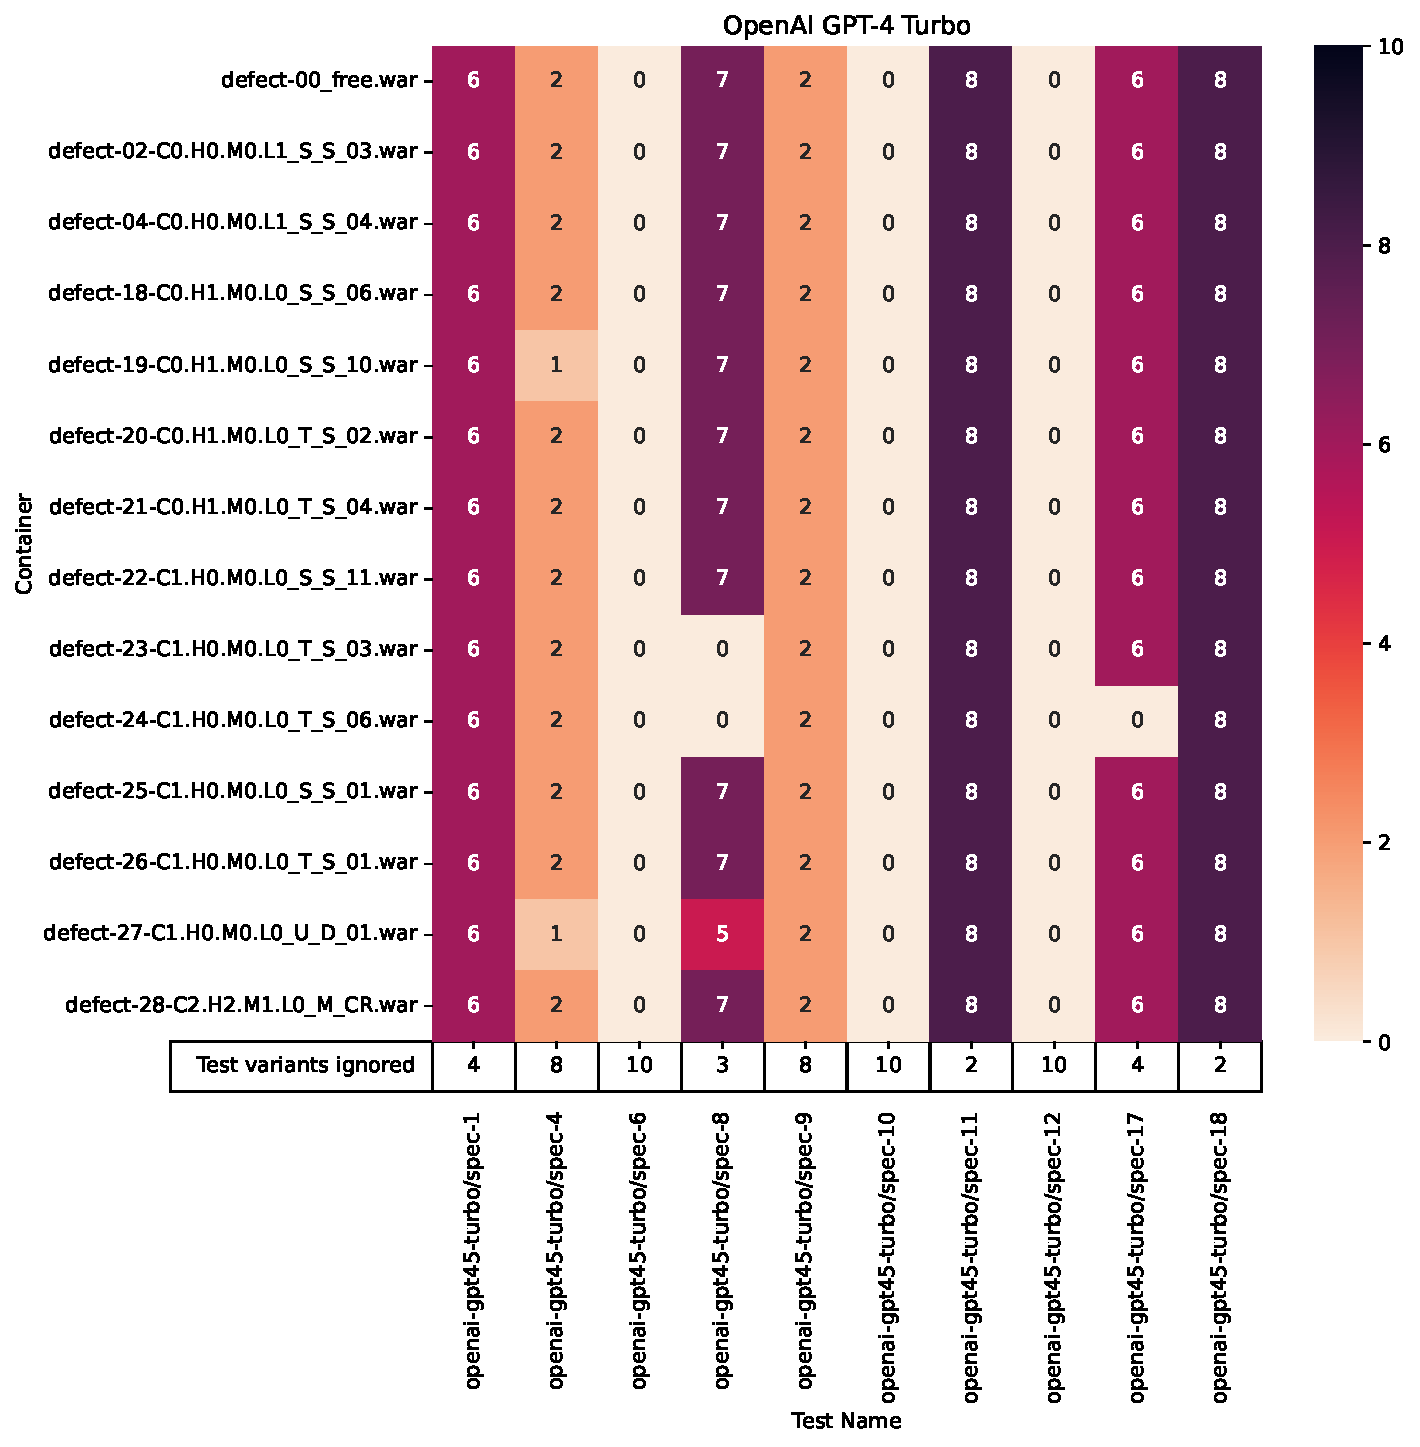
\includegraphics[width=\textwidth]{pic/gpt-4-turbo-results.pdf}
                \caption{Výsledky pro model GPT-4 Turbo}
                \label{fig:res:gpt-4-turbo}
            \end{figure}

            \begin{figure}
                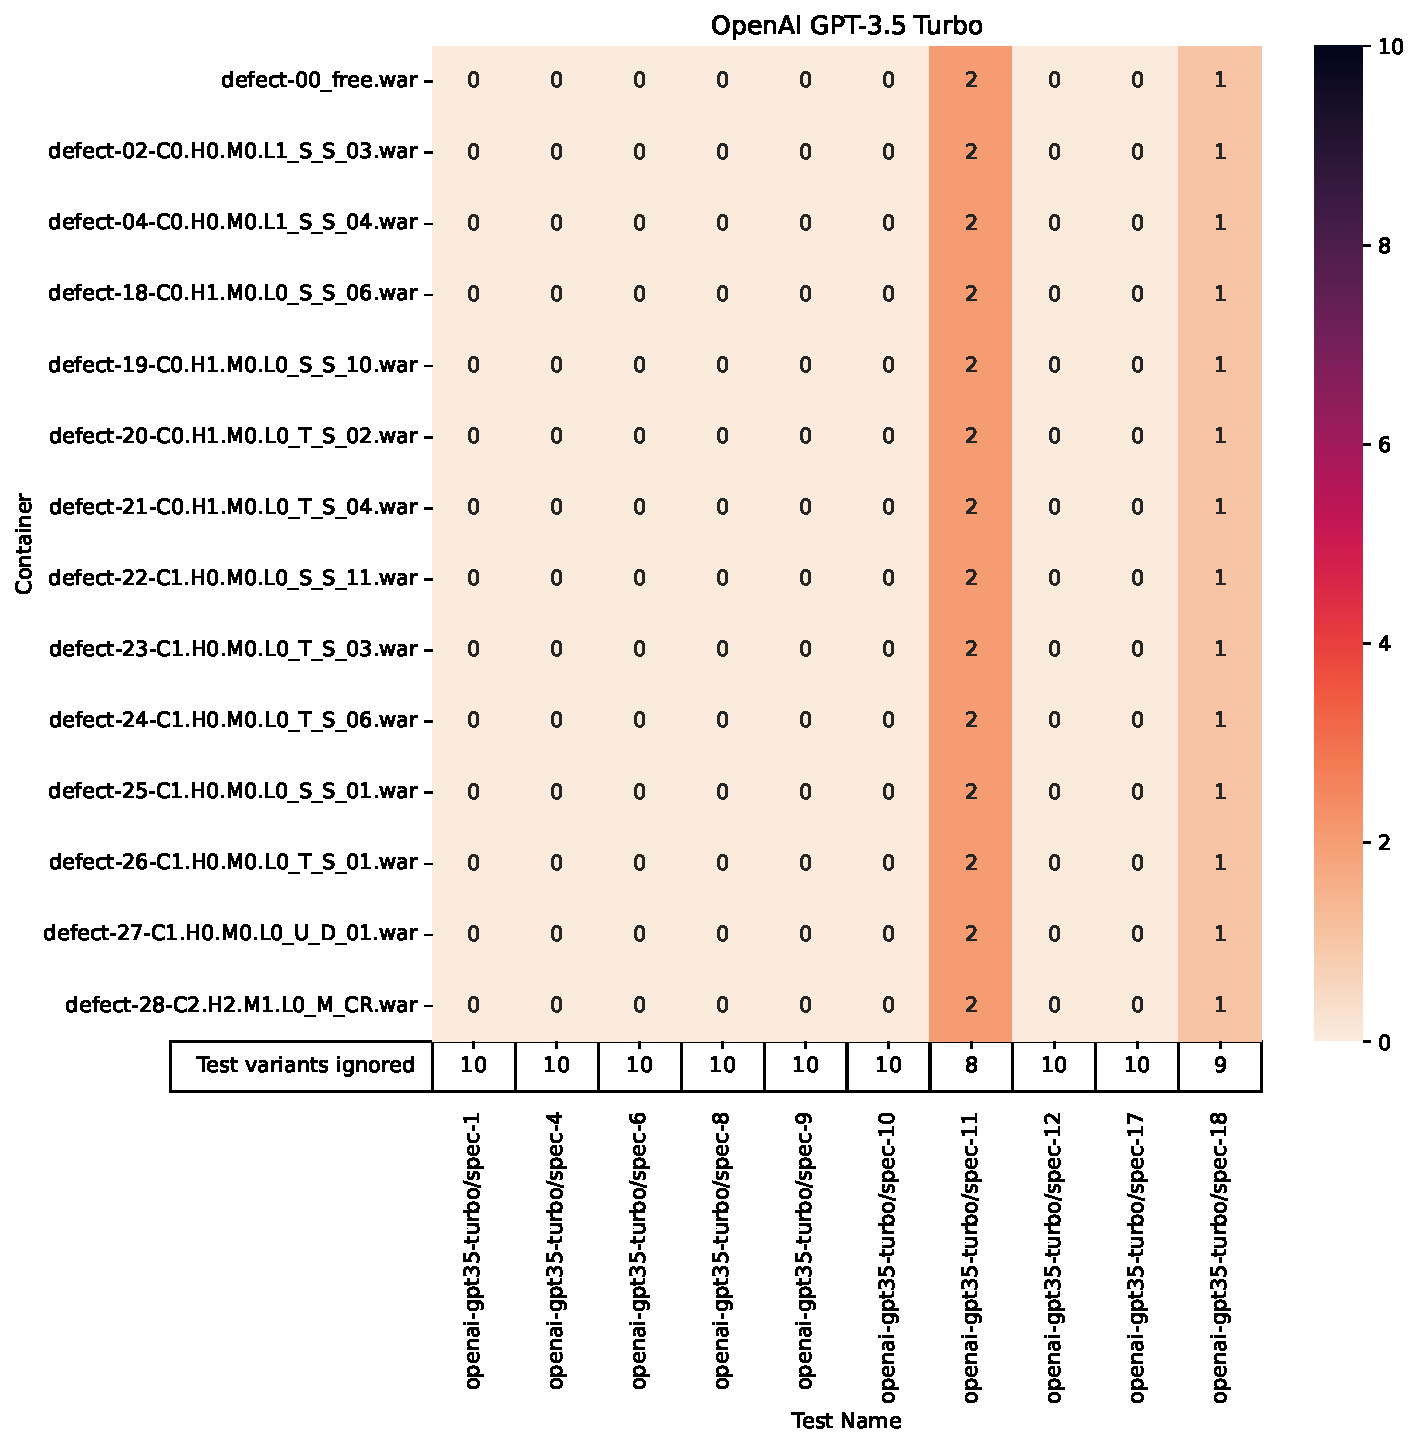
\includegraphics[width=\textwidth]{pic/gpt-3.5-turbo-results.pdf}
                \caption{Výsledky pro model GPT-3.5 Turbo}
                \label{fig:res:gpt-35-turbo}
            \end{figure}

        \subsection{Anthropic}

            \begin{figure}
                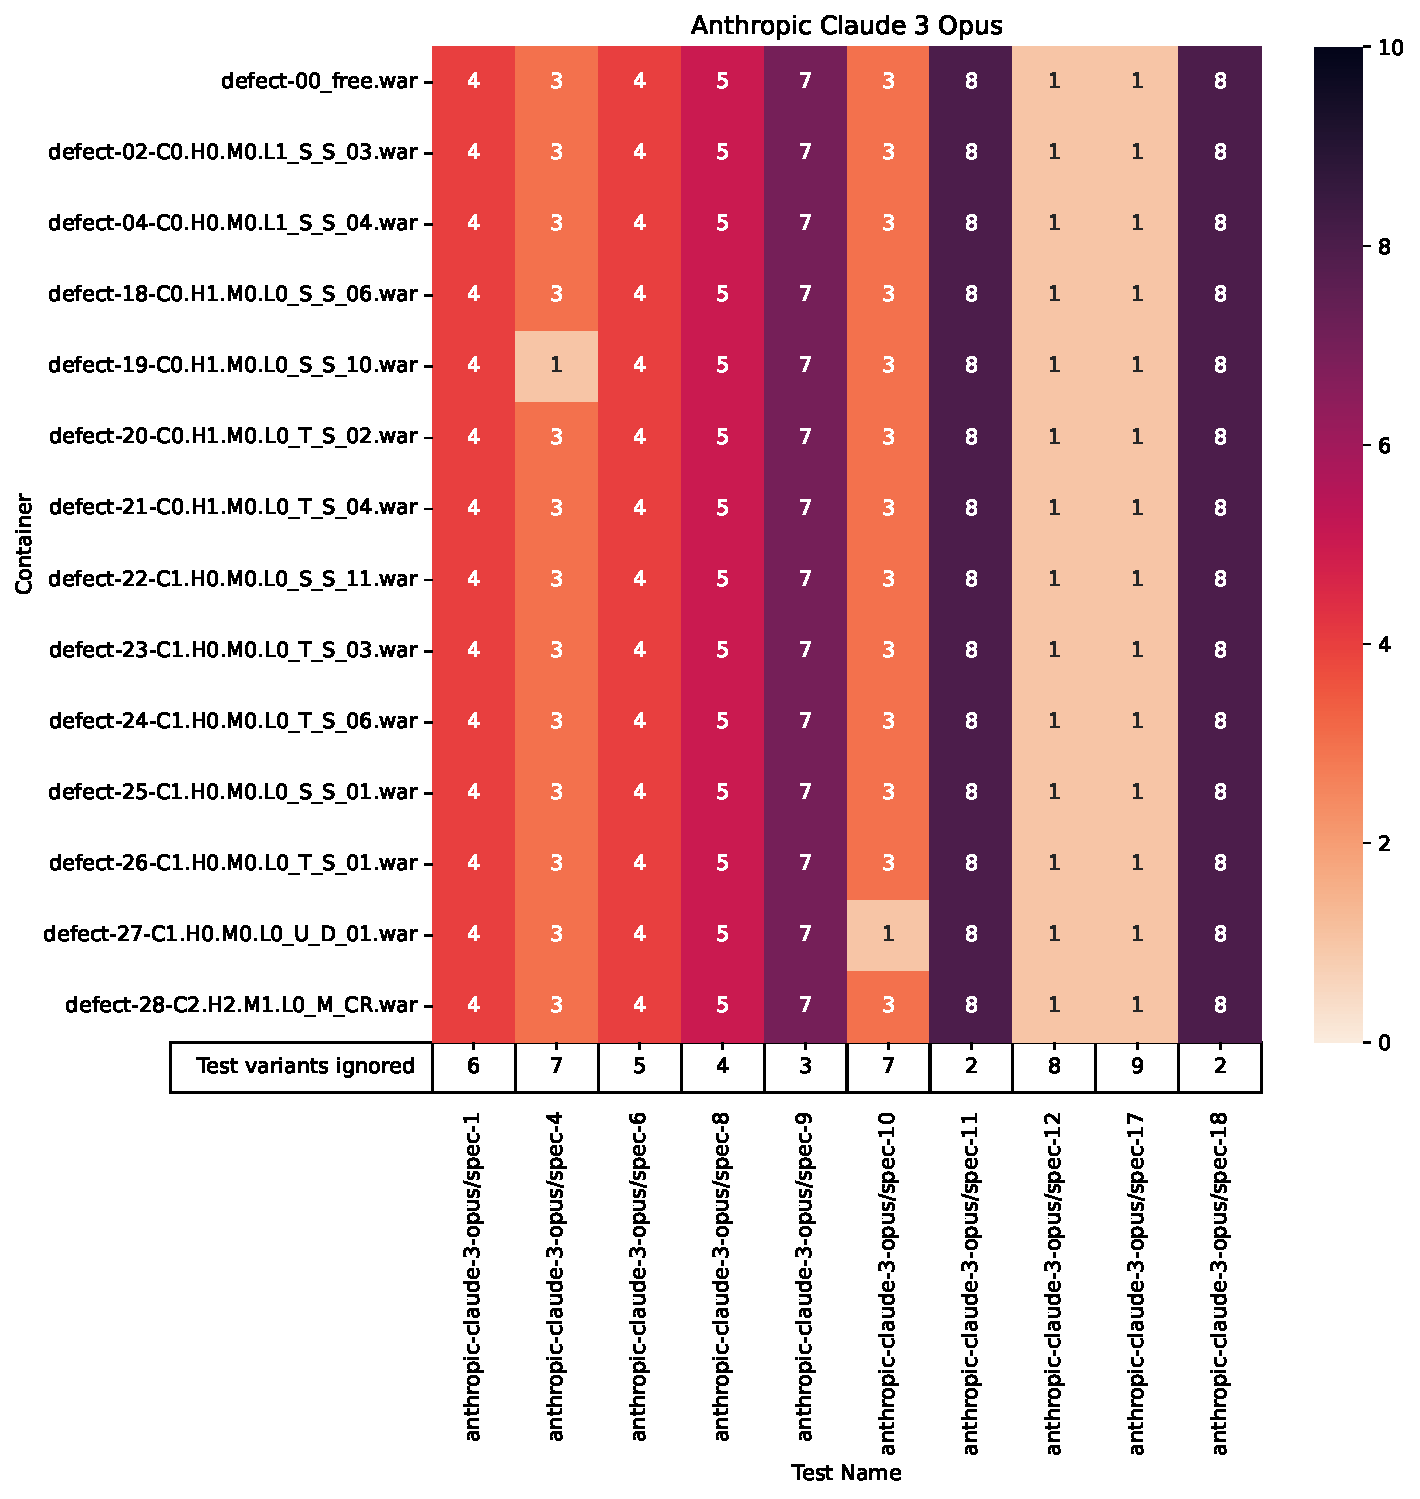
\includegraphics[width=\textwidth]{pic/claude-3-opus-results.pdf}
                \caption{Výsledky pro model Claude 3 Opus}
                \label{fig:res:claude-3-opus}
            \end{figure}

        \subsection{Meta}

        \subsection{Google}

            \begin{figure}
                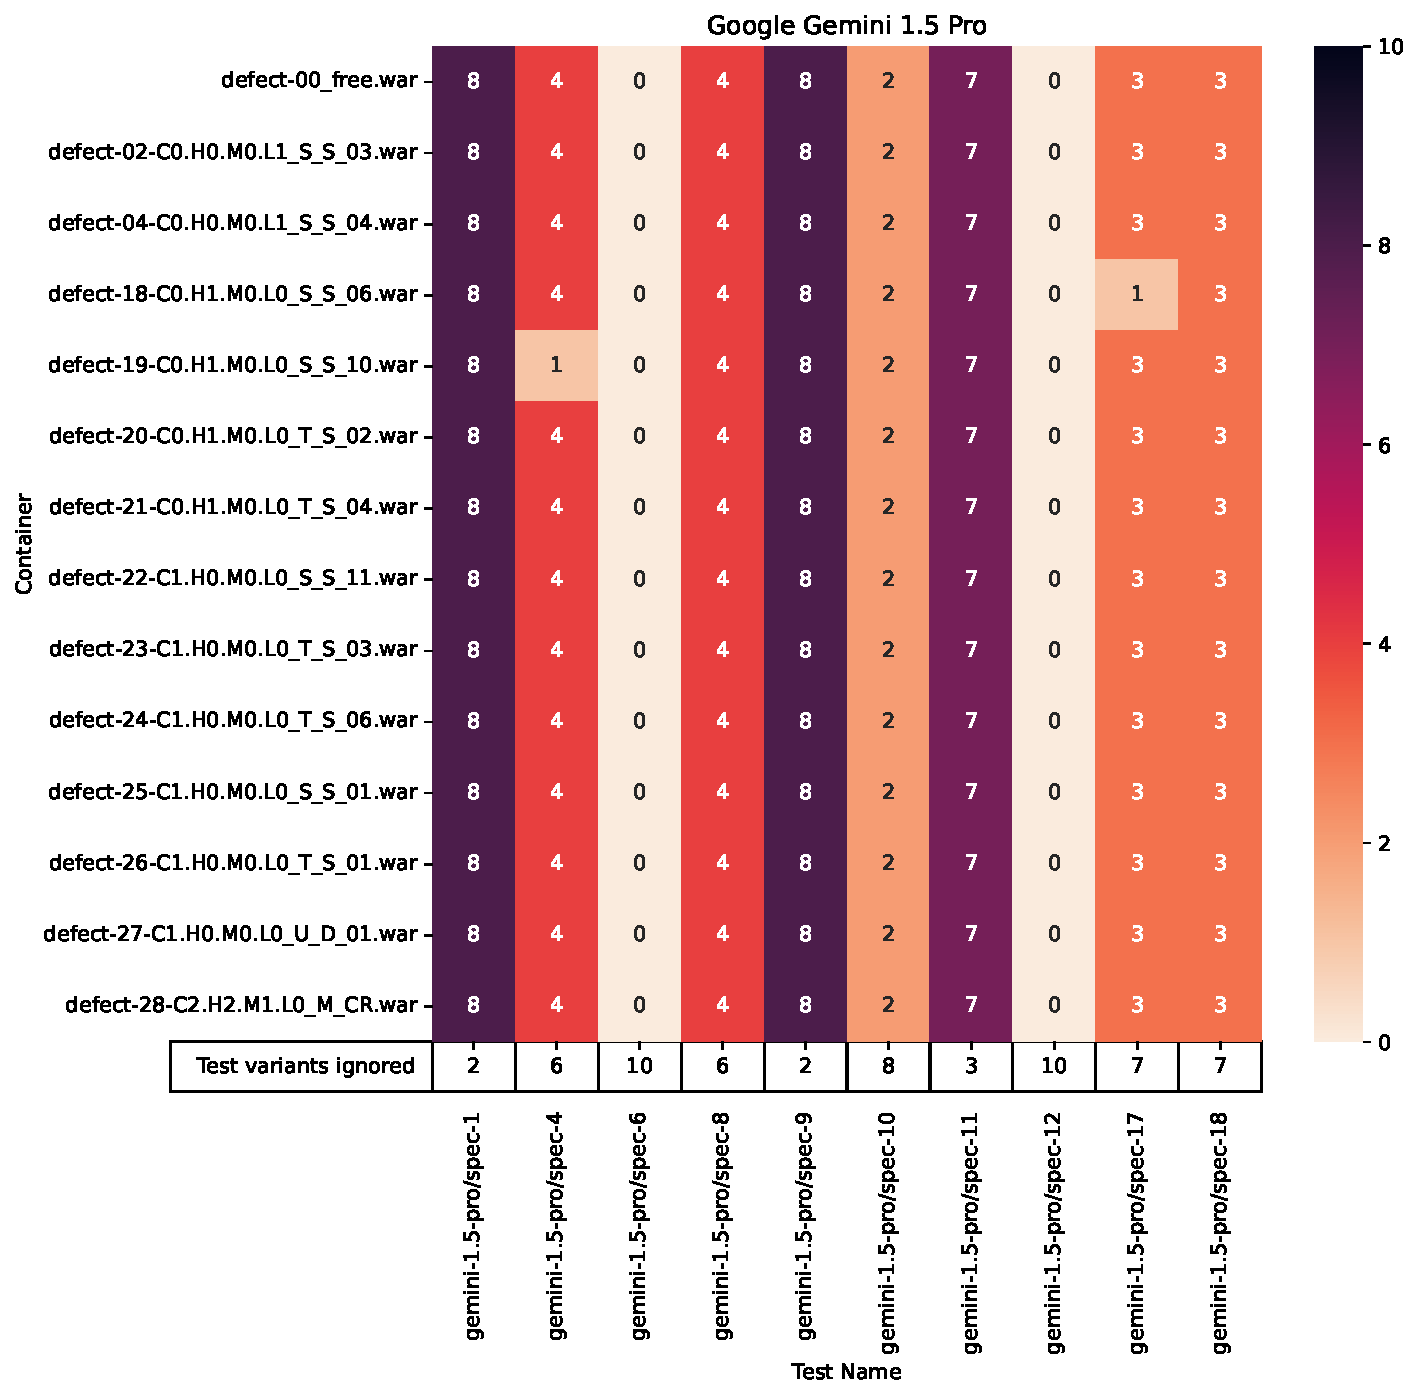
\includegraphics[width=\textwidth]{pic/gemini-results.pdf}
                \caption{Výsledky pro model Google Gemini 1.5 Pro}
                \label{fig:res:gemini}
            \end{figure}

        \subsection{Mistral}

    \section{Cena a časová náročnost generování}
    %TODO Je tohle dobré mít tady?

\chapter{Budoucí vylepšení}
    %TODO Jak snížit cenu - kratší prompty, komprese, atd.

\chapter{Závěr}

% _____________________________________________________________________________
%
%
%        BACK MATTER (BIBLIOGRAPHY, LISTS, ...)
%
% _____________________________________________________________________________
%
\backmatter
\printbibliography
\listoffigures
\listoftables
\listoflistings
% _____________________________________________________________________________
%
%		BACK COVER
% _____________________________________________________________________________
%
%\setbackpagepic{img/fav} % <== an example of one possible option (read this manual)
%\setqrcodebaseurl{https://mycloud.org/show=pdf&docid=} % <== another example
%\setbackpageqrcode{54321} % <== and one more (uncomment the one that makes sense for you)
\setbackpageqrcode
\backpage
\end{document}
